\documentclass[12pt]{article}
\usepackage[swedish,english]{babel}
\usepackage[utf8x]{inputenc}
\usepackage{amsmath}
\usepackage{graphicx}
\usepackage{float} %for insert graph
\usepackage{lscape}
\usepackage{rotating}
\usepackage[colorinlistoftodos]{todonotes}
%\usepackage[margin=1in]{geometry} %set page margin
\usepackage[bottom=1.25in, top=1.25in]{geometry}
%\addtolength{\topmargin}{0.25in}
%\addtolength{\bottommargin}{0.25in}
\usepackage{hyperref} %insert to link to email address
\usepackage{setspace}
\setlength\parindent{24pt} %set indentation
\usepackage{amssymb} %for maths symbols
\usepackage{cases} %for numbering in cases
  %define matlab style
\usepackage{listings}
\usepackage{color} %red, green, blue, yellow, cyan, magenta, black, white
\definecolor{mygreen}{RGB}{28,172,0} % color values Red, Green, Blue
\definecolor{mylilas}{RGB}{170,55,241}

\lstset{language=Matlab,%
    %basicstyle=\color{red},
    breaklines=true,%
    morekeywords={matlab2tikz},
    keywordstyle=\color{blue},%
    morekeywords=[2]{1}, keywordstyle=[2]{\color{black}},
    identifierstyle=\color{black},%
    stringstyle=\color{mylilas},
    commentstyle=\color{mygreen},%
    showstringspaces=false,%without this there will be a symbol in the places where there is a space
    numbers=left,%
    numberstyle={\tiny \color{black}}% size of the numbers
    %numbersep=9pt, % this defines how far the numbers are from the text
    %emph=[1]{for,end,break},emphstyle=[1]\color{red}, %some words to emphasise
    %emph=[2]{word1,word2}, emphstyle=[2]{style},    
}


\begin{document}

%%%%%%%%%%%
%%TITLE PAGE%%%
%%%%%%%%%%%%
\begin{titlepage}

\newcommand{\HRule}{\rule{\linewidth}{0.5mm}} % Defines a new command for the horizontal lines, change thickness here

\center % Center everything on the page
 
%----------------------------------------------------------------------------------------
%   HEADING SECTIONS
%----------------------------------------------------------------------------------------
%Logo First
%----------------------------------------------------------------------------------------
%   LOGO SECTION
%----------------------------------------------------------------------------------------


\includegraphics{UU_logo.eps}\\[0.5cm] % Include a department/university logo - this will require the graphicx package
 
\textsc{\Large Modelling complex systems}\\[0.5cm] % Major heading such as course name


%----------------------------------------------------------------------------------------
%   TITLE SECTION
%----------------------------------------------------------------------------------------

\HRule \\[0.4cm]
{\huge \bfseries Project 1: \par A firing brain \& Spread of memes }\\[0.4cm] % Title of your document
\HRule \\[1.5cm]
 
%----------------------------------------------------------------------------------------
%   AUTHOR SECTION
%----------------------------------------------------------------------------------------

{\huge Peili Guo\\} %insert your name 
{\large \href{mailto:Peili.Guo.7645@student.uu.se}{Peili.Guo.7645@student.uu.se}}
\\[2cm] %insert page break length

%----------------------------------------------------------------------------------------
%   DATE SECTION
%----------------------------------------------------------------------------------------

{\Large \today}\\[2cm] % Date, change the \today to a set date if you want to be precise


%----------------------------------------------------------------------------------------

\vfill % Fill the rest of the page with whitespace

\end{titlepage}

\newpage
%%%%%%%%%%%%
%%%start report 
%%%1. fire brain
%%%%%%%%%%%

\section{A firing brain}
\doublespacing
In this part, a simple program in matlab was written to simulate a firing brain with two-dimensional cellular automata model on a N by N grid with periodic boundary conditions.\par

each grid represents a neuron. there are 3 different states for neuron: ready(0), firing(1), and resting(2). 
the rules for transit to the next time steps are:

\begin{enumerate}
\item a ready neuron fires on the next time step if there are exactly two neighbours that are firing. ( 0 $\rightarrow$ 1, if two neighbours are 1).
\item a firing neuron goes to the resting state on the next time step (1 $\rightarrow$ 2).
\item a firing neuron goes to ready state on the next time step (2 $\rightarrow$ 0).
\end{enumerate}


\subsection{simple simulation in matlab}

Below are the results for a 40 x 40 grid where initially each cell has a probability of 0.3 being a firing(1) cell and all other neurons are ready. the figures below shows how the cells looks like after 10, 20, 100 and 1000 time steps. 

The initial probability of being in a firing state is 0.3, which means at t = 0, there are around 480 cells that are being in a firing state. as we can see in figure \ref{fig:100sim}, the total number of firing cell decreases over time. In the beginning, the number of cell decreases very fast, and the total number of cells gets stable around t = 300~400. When simulate 100 times to t = 1000, the average firing cell at t = 400 is around 14 and at t = 1000, the average firing cell is around 12. At the equilibrium state, the shapes that remains are travelling forward at a constant rate preserving the same shape either in the same direction(up/down or left/right), or will never interact if there are shape that travel in the up/down direction and others in left/right direction. Over 100 simulation, the curve of average firing cell decreases in an exponential model, and a exponential model of y = a* exp(b*x) + c*exp(d*x) was fitted to the curve in figure \ref{fig:sim_model}.


\begin{figure}[H] %figure 1 at t=10
\centering
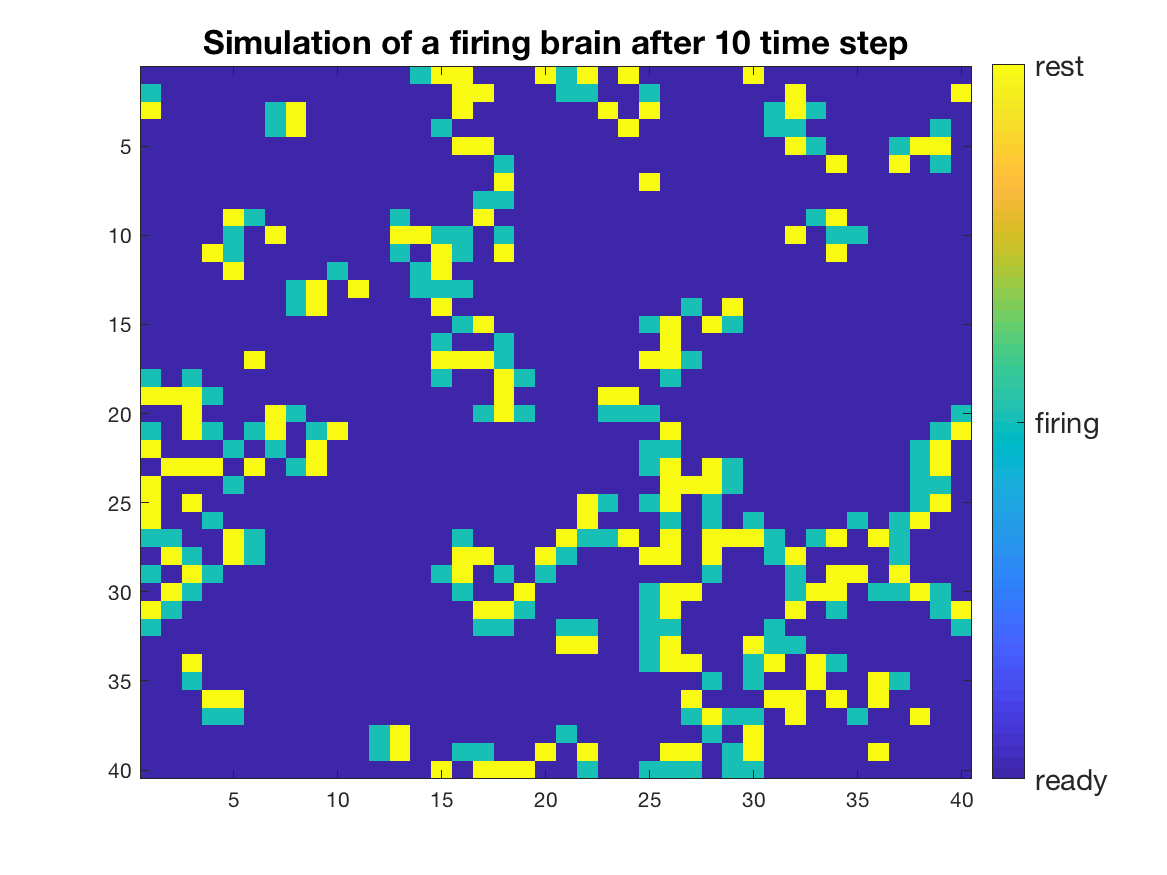
\includegraphics[width = 12 cm, height = 9cm]{fire10.png}
\caption{40x40 cell grid at t = 10}
\label{fig:fire10}
\end{figure}

\begin{figure}[H] %figure 1 at t=20
\centering
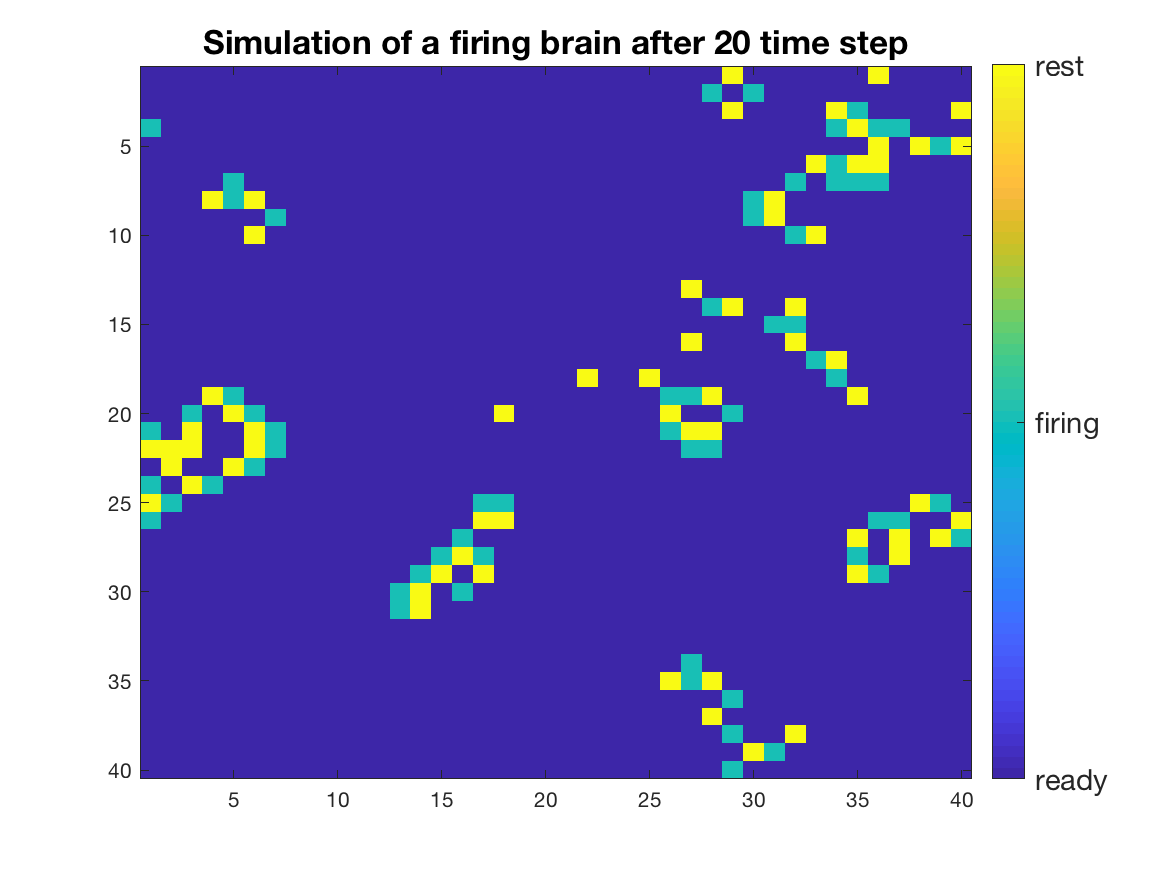
\includegraphics[width = 12 cm, height = 9cm]{fire20.png}
\caption{40x40 cell grid at t = 20}
\label{fig:fire20}
\end{figure}

\begin{figure}[H] %figure 1 at t=100
\centering
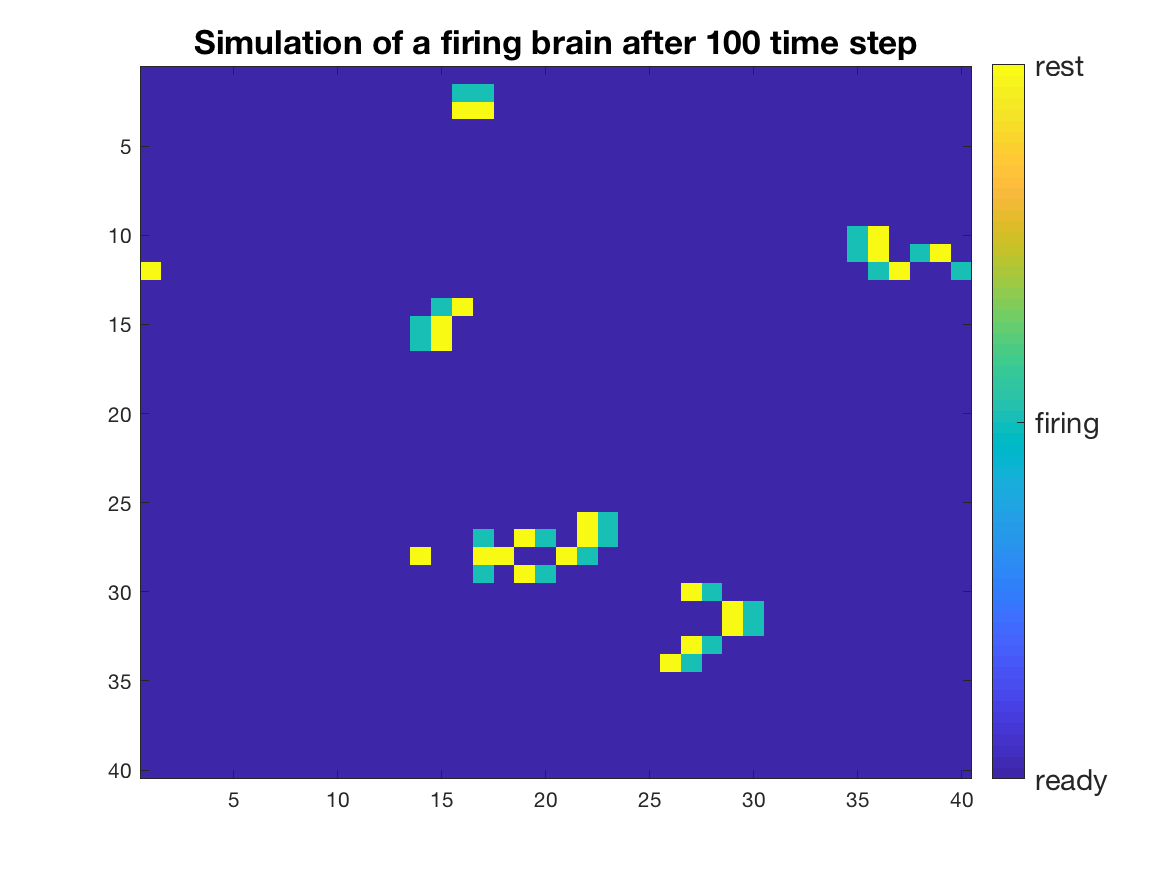
\includegraphics[width = 12 cm, height = 9cm]{fire100.png}
\caption{40x40 cell grid at t = 100}
\label{fig:fire100}
\end{figure}

\begin{figure}[H] %figure 1 at t=1000
\centering
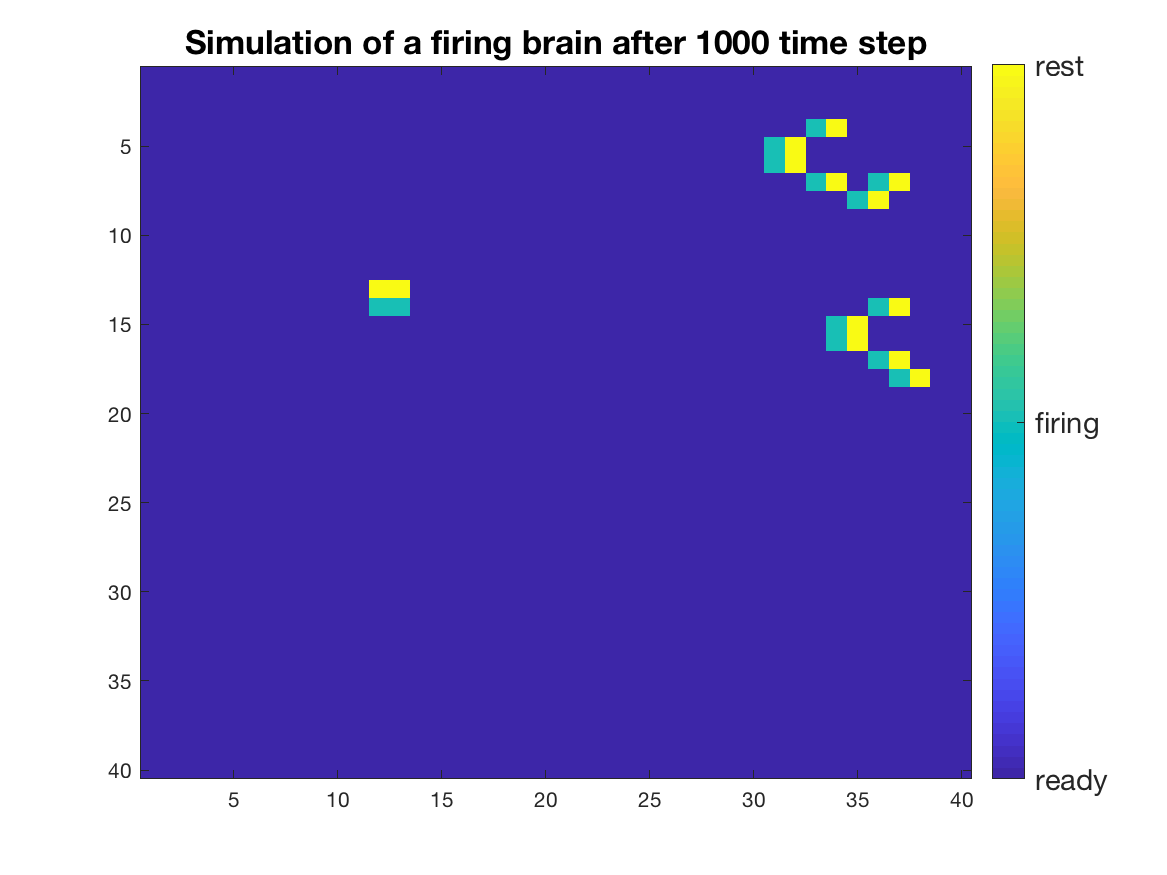
\includegraphics[width = 12 cm, height = 9cm]{fire1000.png}
\caption{40x40 cell grid at t = 1000}
\label{fig:fire1000}
\end{figure}

\begin{figure}[H] %figure 1 at t=1000
\centering
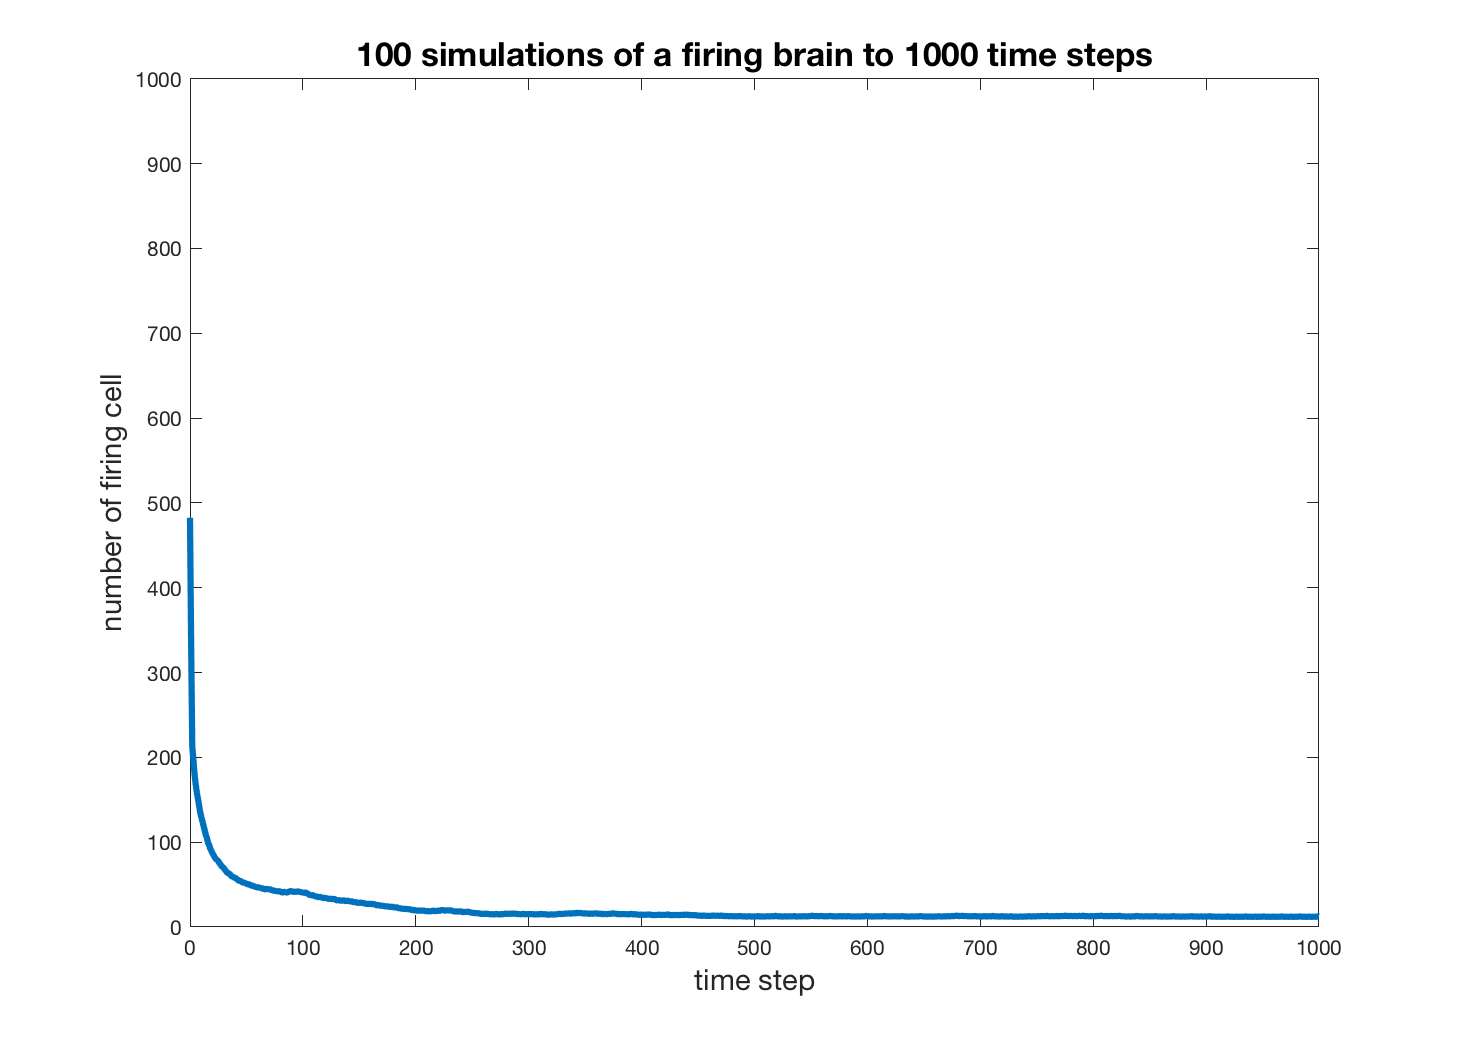
\includegraphics[width = 12 cm, height = 9cm]{firebrain100sim.png}
\caption{average number of firing cells over time with 100 simulation of different initial conditions}
\label{fig:100sim}
\end{figure}

\begin{figure}[H] %model fit
\centering
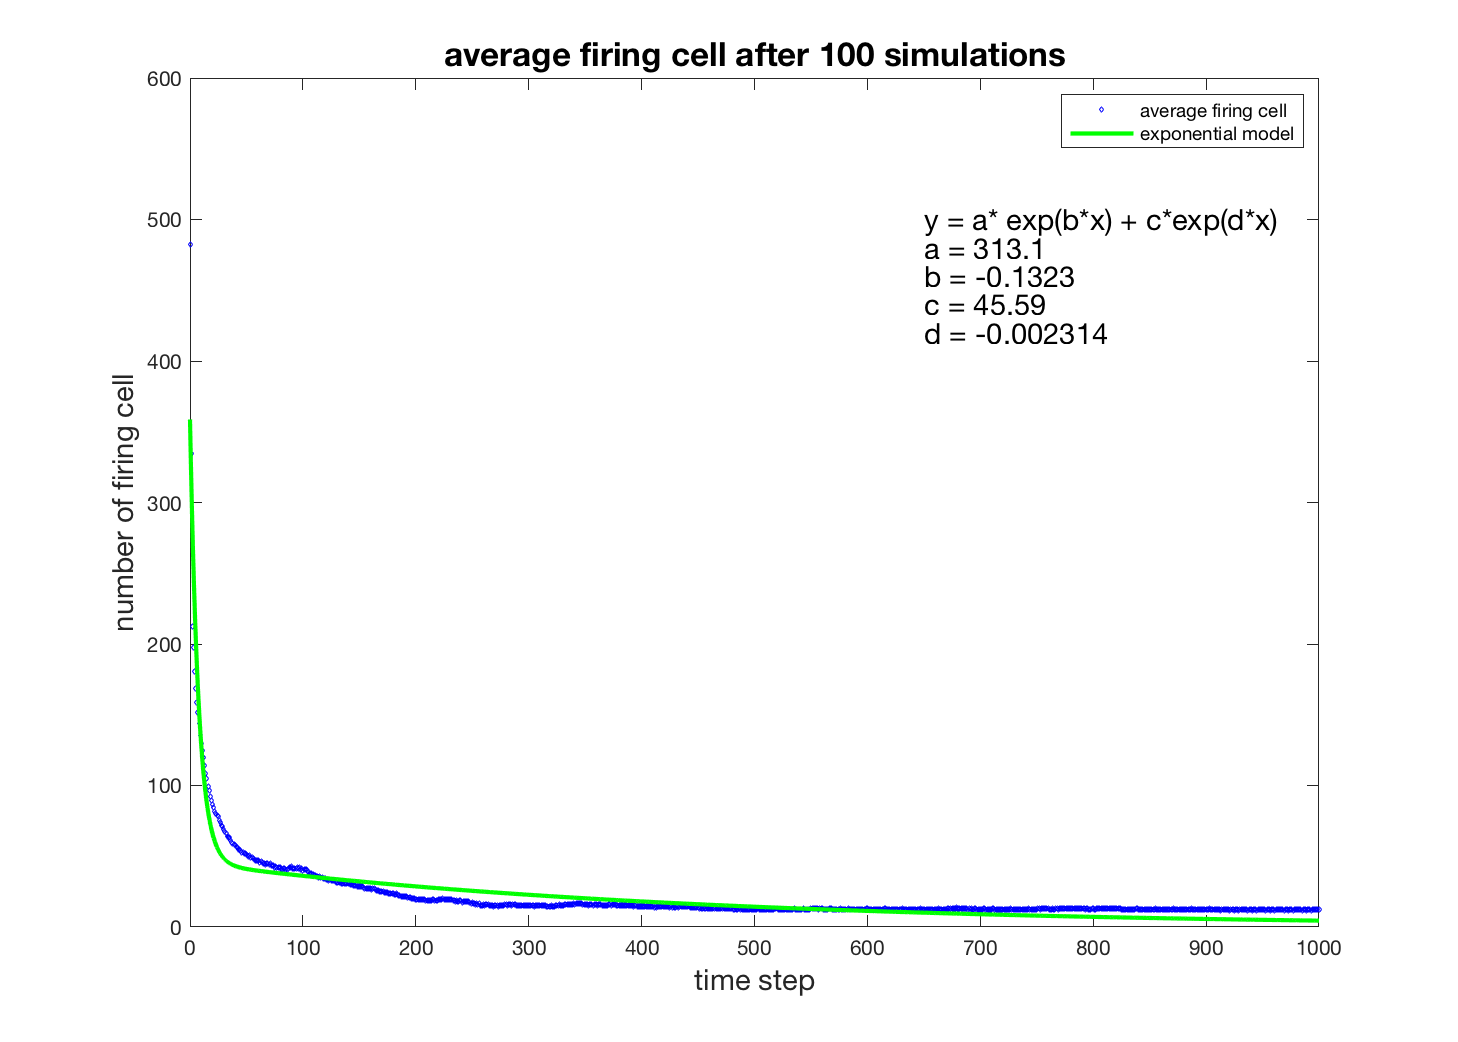
\includegraphics[width = 12 cm, height = 9cm]{sim_model.png}
\caption{average number of firing cells over time with 100 simulation and exponential model fitting}
\label{fig:sim_model}
\end{figure}

and here are the links of video you can check out.\par 
for simulation to t = 100\par
\url{<https://youtu.be/CFUcpGHhj00>}\par
for simulation to t = 1000\par
\url{<https://youtu.be/8EulLy_IRmw>}\par

%%%%%%%%%%%finish 1.1 %%%%%%%%%%%%


%%%%%%%%%% start 1.2%%%%%%%%%%%%%%

\subsection{example of shapes}

\subsubsection{move forward at a rate of one cell per time step, while preserving the same shape}
\begin{figure}[H] %move forward space ship
\centering
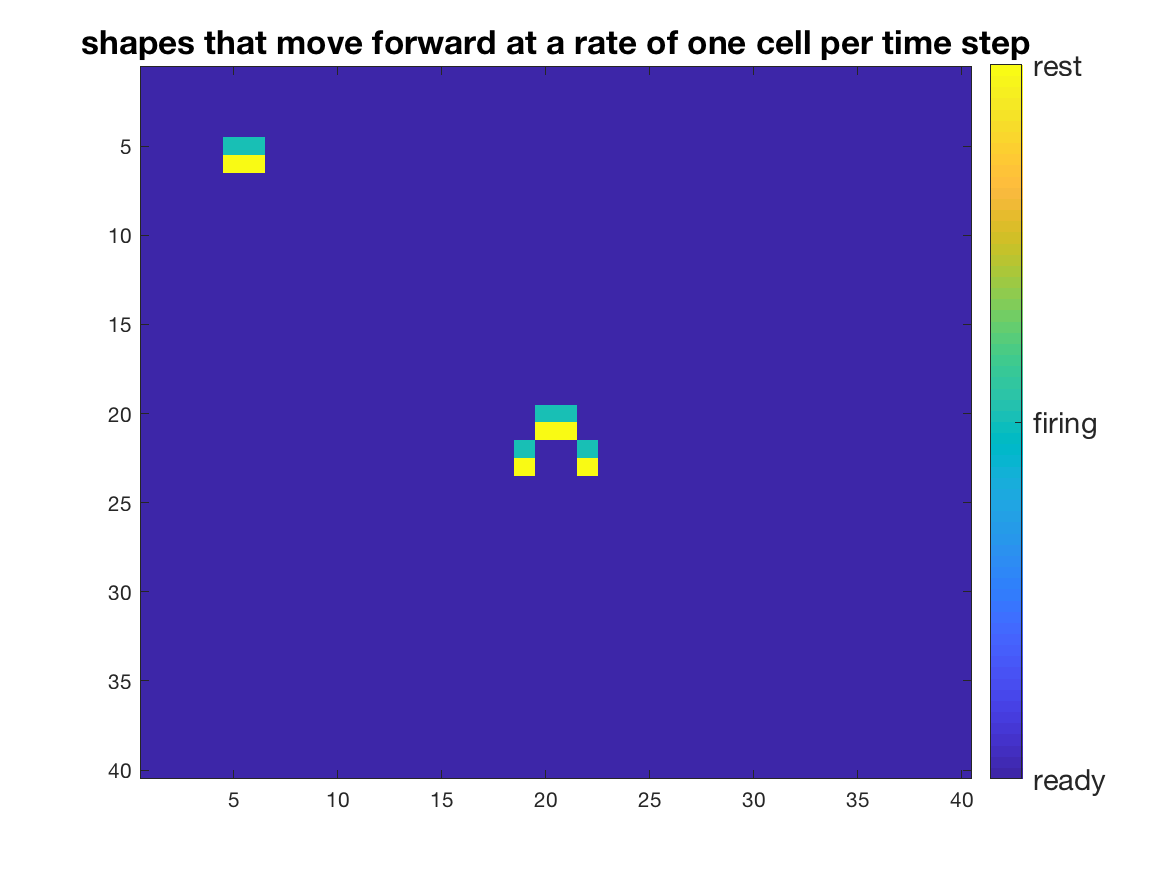
\includegraphics[width = 16 cm, height = 13cm]{task2_1.png}
\caption{shapes that move forward at a rate of one cell per time step preserving the same shape}
\label{fig:task2_1}
\end{figure}

\subsubsection{move forward at a rate of one cell per time step, launching other shapes behind them}
\begin{figure}[H] %launch other shapes
\centering
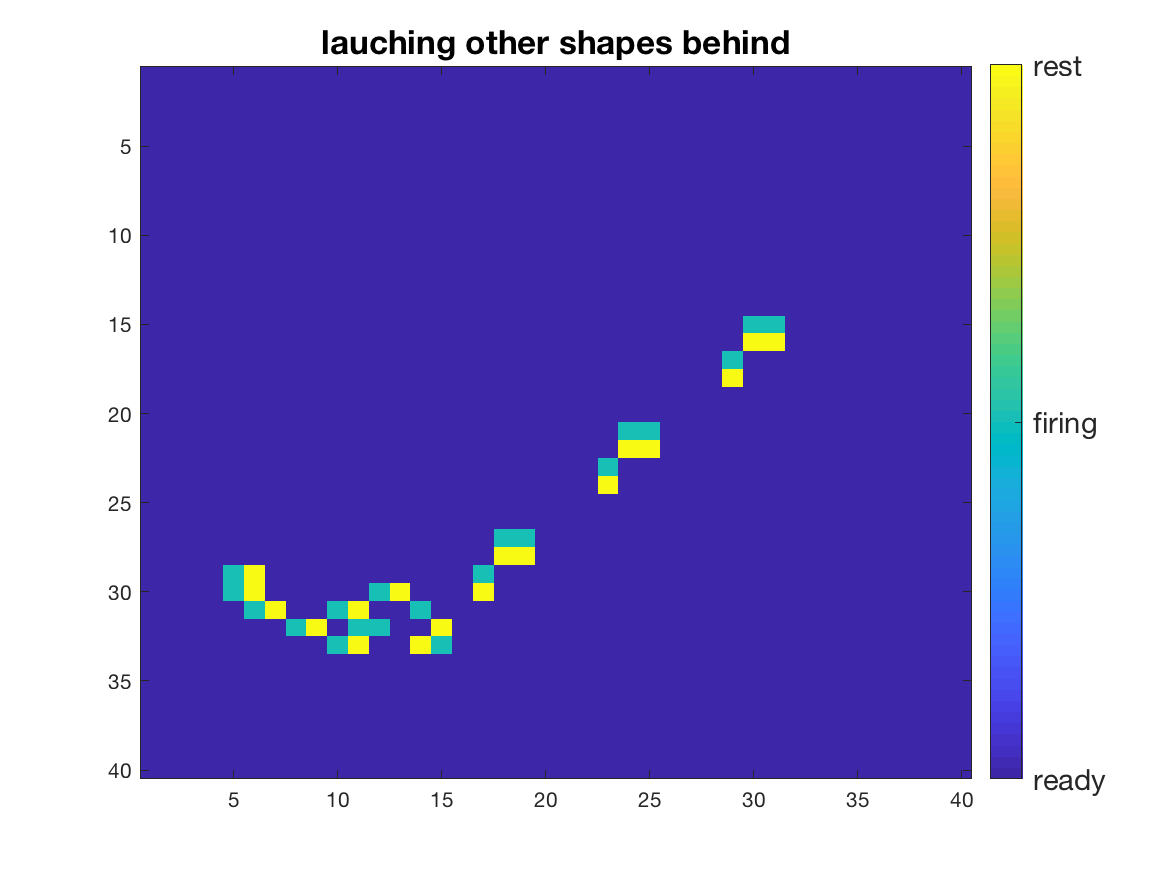
\includegraphics[width = 16 cm, height = 13cm]{task2_2.png}
\caption{shapes that move forward at a rate of one cell per time step, launching other shapes behind them}
\label{fig:task2_2}
\end{figure}

\subsubsection{move forward at a rate of less than one cell per time step, while returning to the same shape after some period}
\begin{figure}[H] %move slower than 1 cell per time
\centering
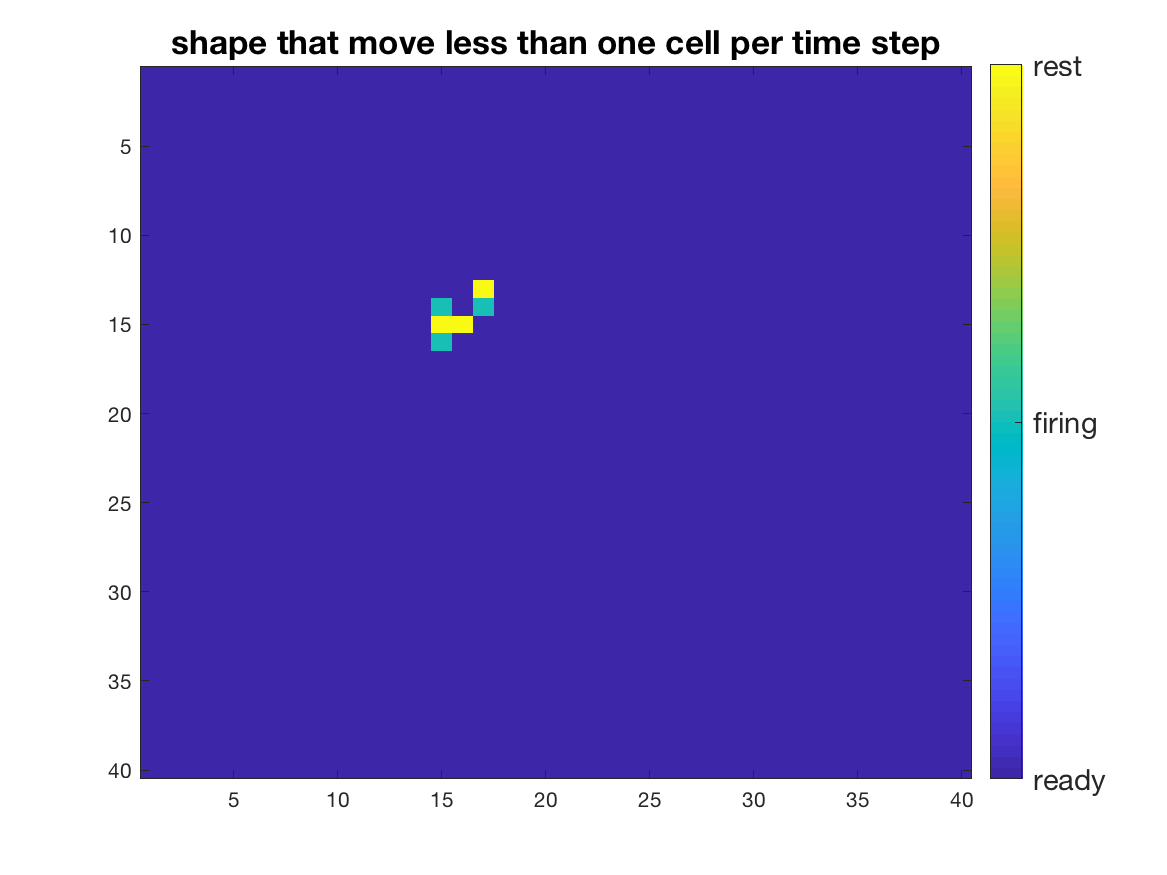
\includegraphics[width = 16 cm, height = 13cm]{task2_3.png}
\caption{shapes that move less than one cell per time step, returning to same shape after some period}
\label{fig:task2_3}
\end{figure}

\subsubsection{stay stationary but oscillate periodically}
\begin{figure}[H] %oscillate
\centering
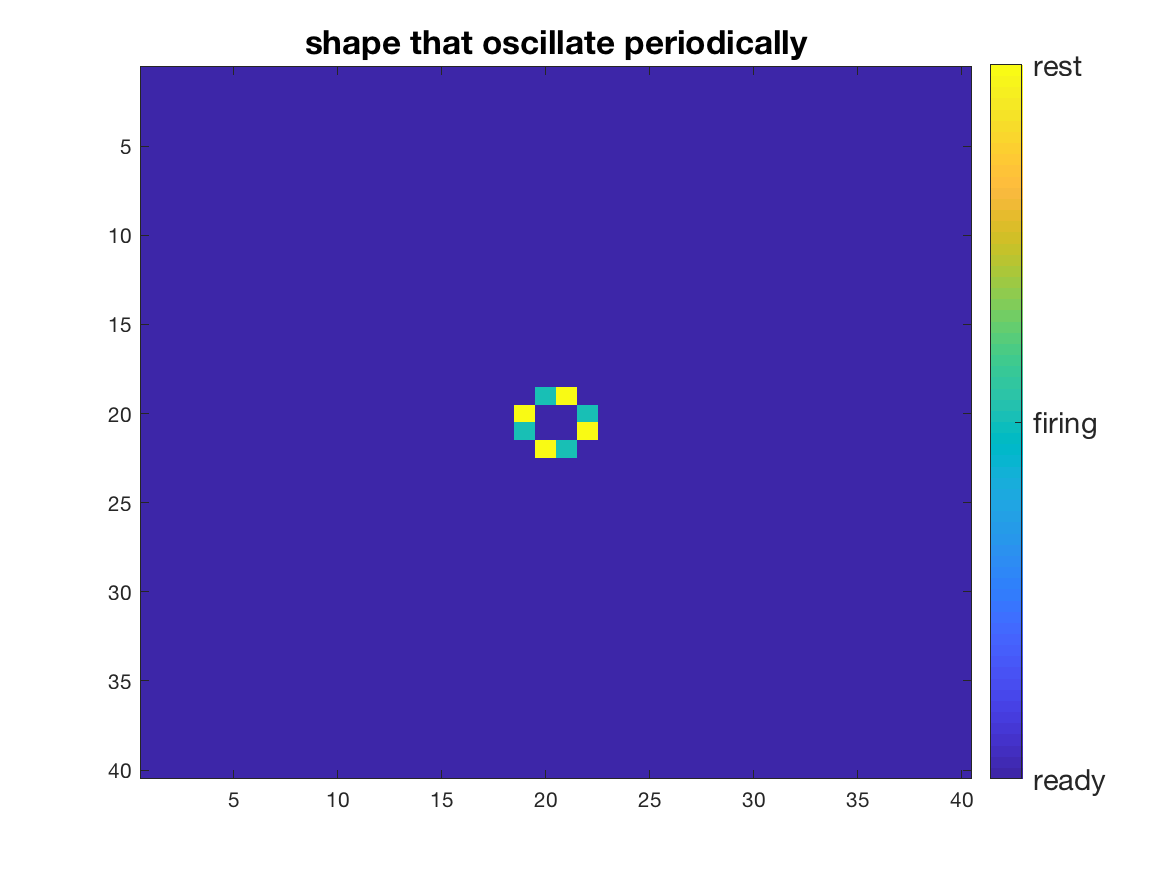
\includegraphics[width = 16 cm, height = 13cm]{task2_4.png}
\caption{shapes that stay stationary but oscillate periodically}
\label{fig:task2_4}
\end{figure}

%%%%%%%%%%%%%end of 1.2

\subsection{create cellular automata}
In this part, I create my own cellular automata. I used the two model in this project (a firing brain and spread of memes), Conway's game of life and several videos I watched online showing cellular automata as reference. I create the following to simulate a population the different life stage.\par
The states are:
\begin{itemize}  
\item Waiting(0)
\item Growing(1)
\item Reproducing(2)
\item Ageing (3)
\item Dead (4)\\
\end{itemize}

The rules for the next time steps are:
\begin{itemize}  
\item The waiting (0) cell needs at least 2 neighbour that are in the stage of reproducing(2) to be in grow. otherwise, it stays waiting.
\item The growing (1) cell needs at least 1 neighbour that is in the stage of reproducing(2) and ageing(3) to become a reproducing (2) cell in the next time step. otherwise, it stays growing.
\item The reproducing(2) celll has the probability of 0.5 to be ageing and 0.5 to remain reproducing
\item The ageing cell (3)has the probability of 0.5 to be dead and 0.5 to remain ageing.
\item The dead cell(4) has the the probability of 0.6 to be in waiting in the next time step, and 0.4 remain dead.
\end{itemize}

To simulate, I set up the initial condition:

\begin{itemize}  
\item each cell has the probability of 0.05 to be a growing cell(1)
\item each cell has the probability of 0.05 to be a reproducing cell(2)
\item each cell has the probability of 0.15 to be in ageing (3)
\item each cell has the probability of 0.10 to be dead(4)
\end{itemize}

I created this to simulate life from a society that is dominated by ageing population. The population will cluster together in the beginning and then different shapes will interact with each other.

\begin{figure}[H] %oscillate
\centering
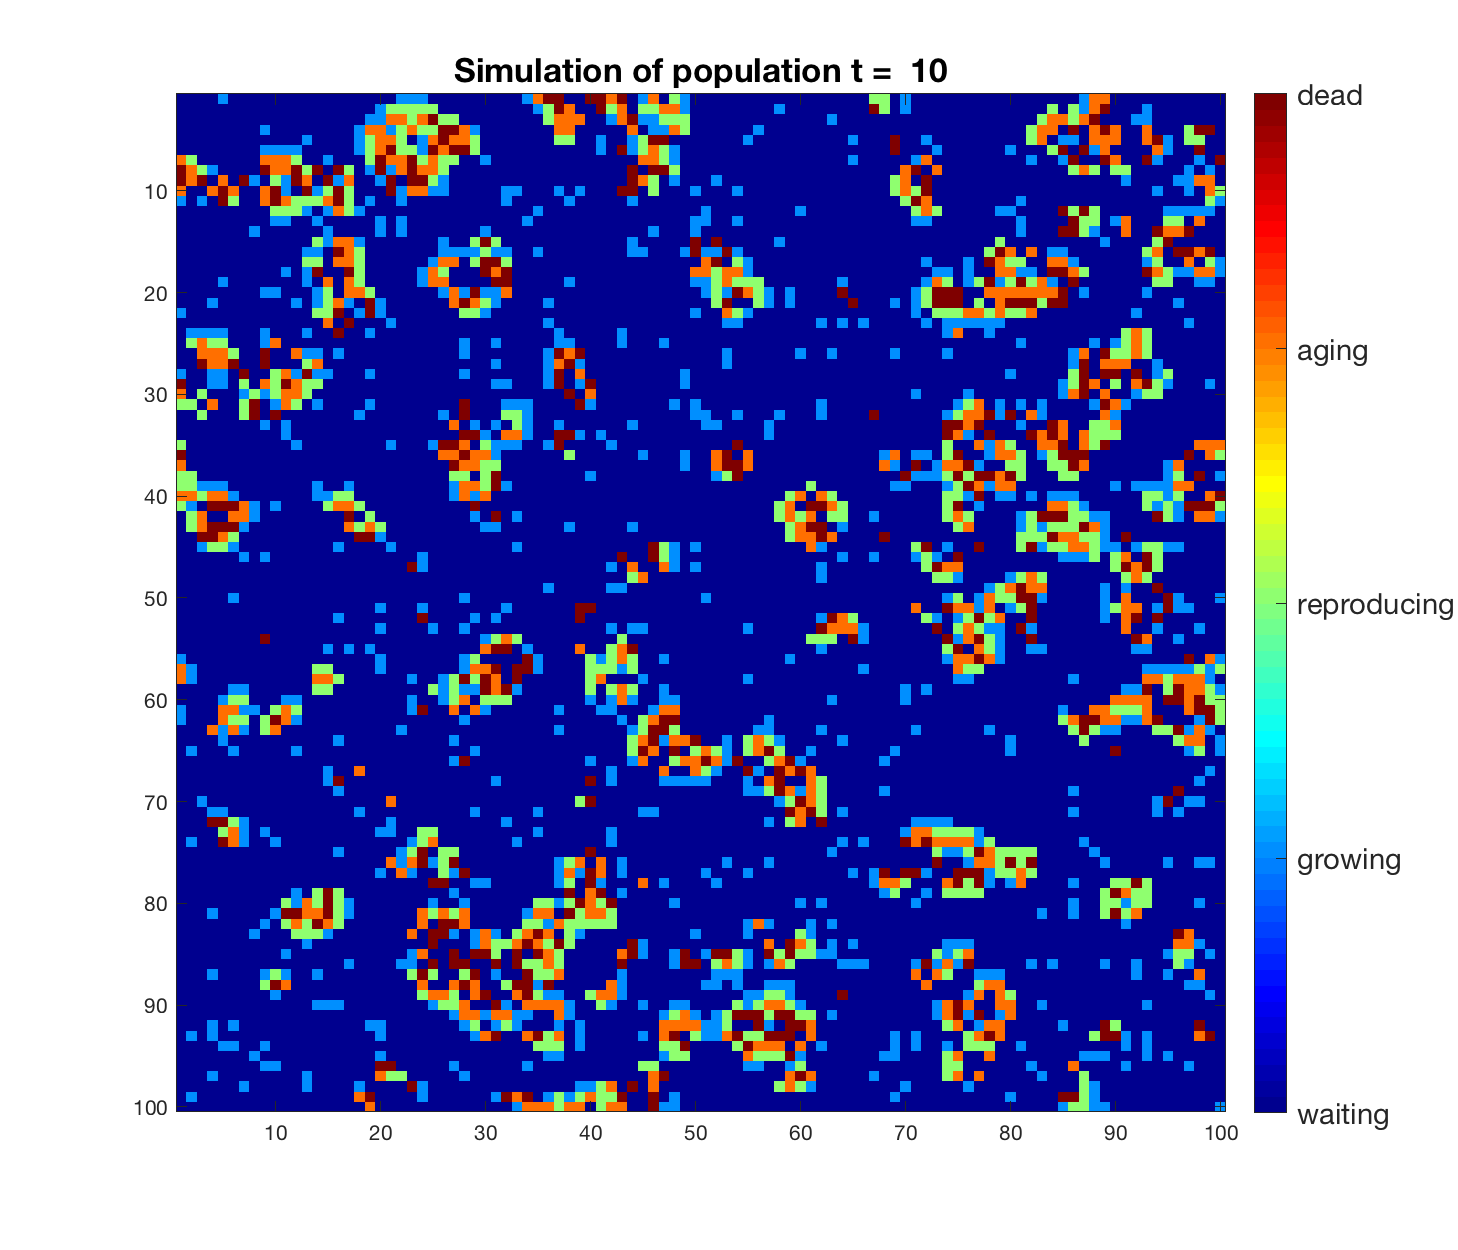
\includegraphics[width = 12 cm, height = 9cm]{mycell_automata.png}
\caption{my cell automata at t = 10}
\label{fig:myca}
\end{figure}

and here are the links of video you can check out.\par 
for simulation to t = 100\par
\url{<https://youtu.be/gQ4c2FFDzDA>}\par
for simulation to t = 1000\par
\url{<https://youtu.be/OWazMF6is1c>}\par



%%%%%%%leave it as now. 
%%%%%%%%%%%%%%%
%%%%%%%%%%%%%%%

%%%%%%%%%%%%%%%
%%%%%%%%%%%%%%%2. memes
\newpage
\section{Spread of memes}
\doublespacing
In this part, a model is used to simulate the spread of internet memes. There are 3 different states, resting(0), sharing(1) and bored(2). The rules for the next time step are:

\begin{enumerate}
\item with probability p = 0.001, a person at rest will discover a new meme and become a sharer.(0 $\rightarrow$ 1 with p = 0.001) 
\item with probability q = 0.01, a person sharing(1) will pick one person completely at random from the population to share the memes with. if the random person is at rest(0), that person will become a sharer(1), if that person is bored(2), then the sharing person will become bored(2). 
\item bored(2) stays bored(2) forever. (2 is always 2).
\end{enumerate}

\subsection{some simulations in matlab}
The simluation in matlab will run the model 1000 times with a population of 1000 to time at 2000 and show the change of number of resting, sharing and bored person over time. The initial condition is that there are one person sharing and one bored person. and below are the graphs showing the simulation. 

\begin{figure}[H] %1000 meme run >.<
\centering
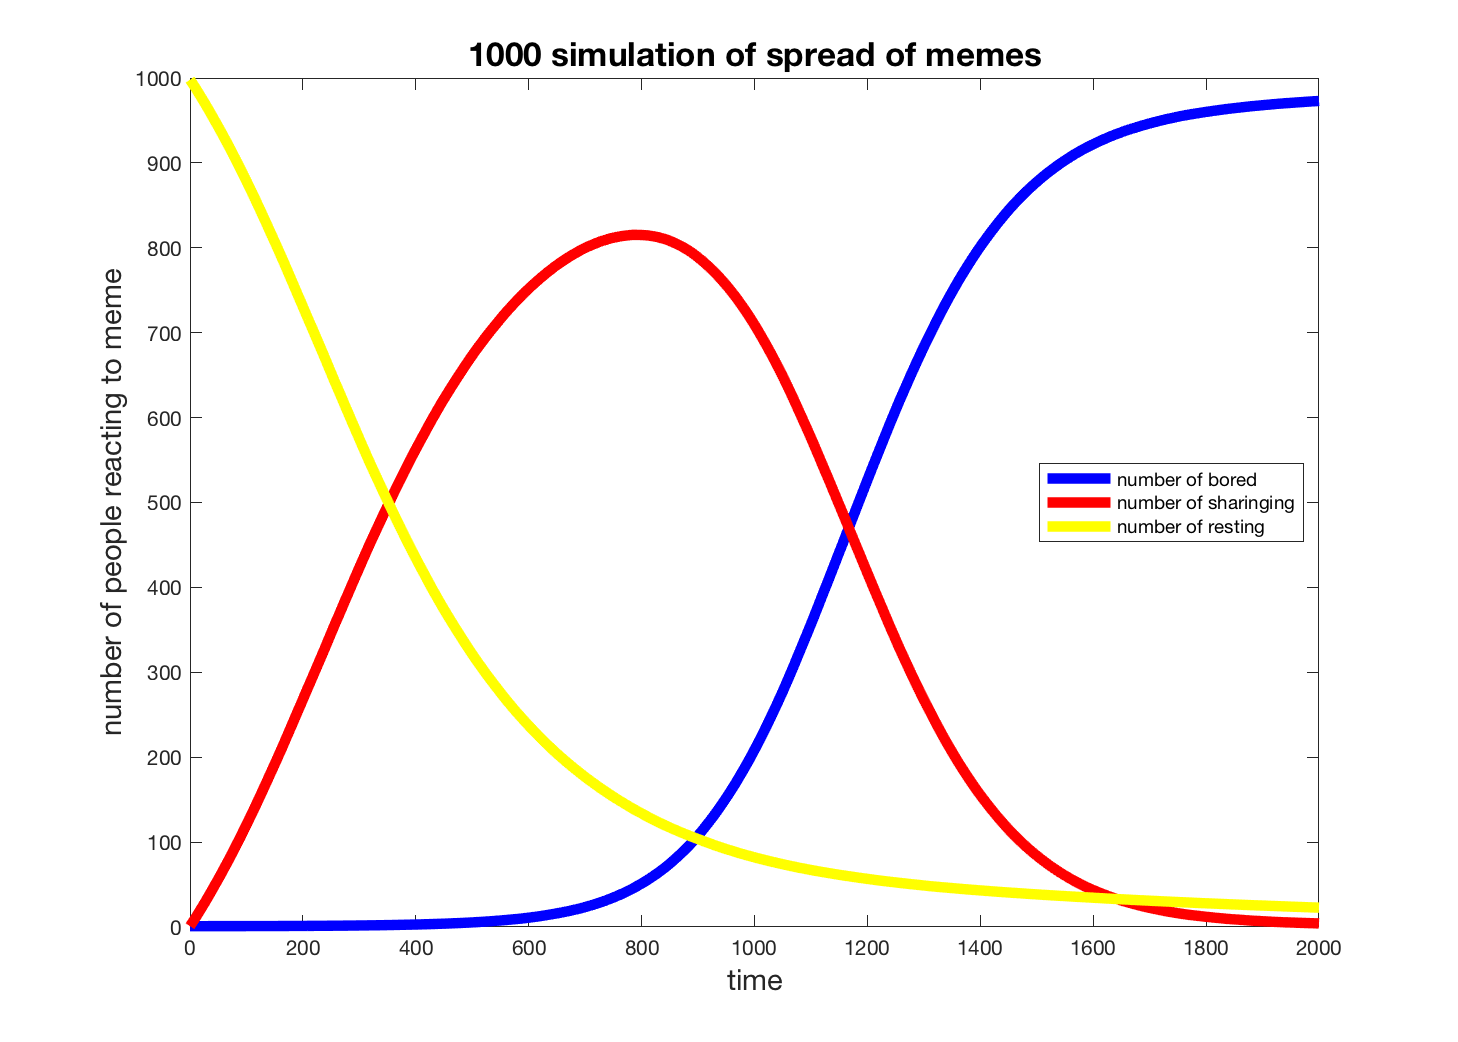
\includegraphics[width = 12 cm, height = 9cm]{memes_sim_1000times.png}
\caption{simulation of spread of memes showing number of bored, sharing, resting person over time}
\label{fig:mem}
\end{figure}

The mean field difference equation model for the sharing of meme is: \par
Bored(B), Sharing(S), Resting(R), population(N).\par
\begin{numcases}{ }
	B(t+1) = B(t) + S(t)*q*B(t)/N\\
	S(t+1) = S(t) + p*R(t) - S(t)*q*B(t)/N + S(t)*q*R(t)/N\\
	R(t+1) = R(t) - R(t)*p - S(t)*q*R(t)/N
\end{numcases}

The figure below shows both the simulation and the mean field model
\begin{figure}[H] %1000 meme run >.<
\centering
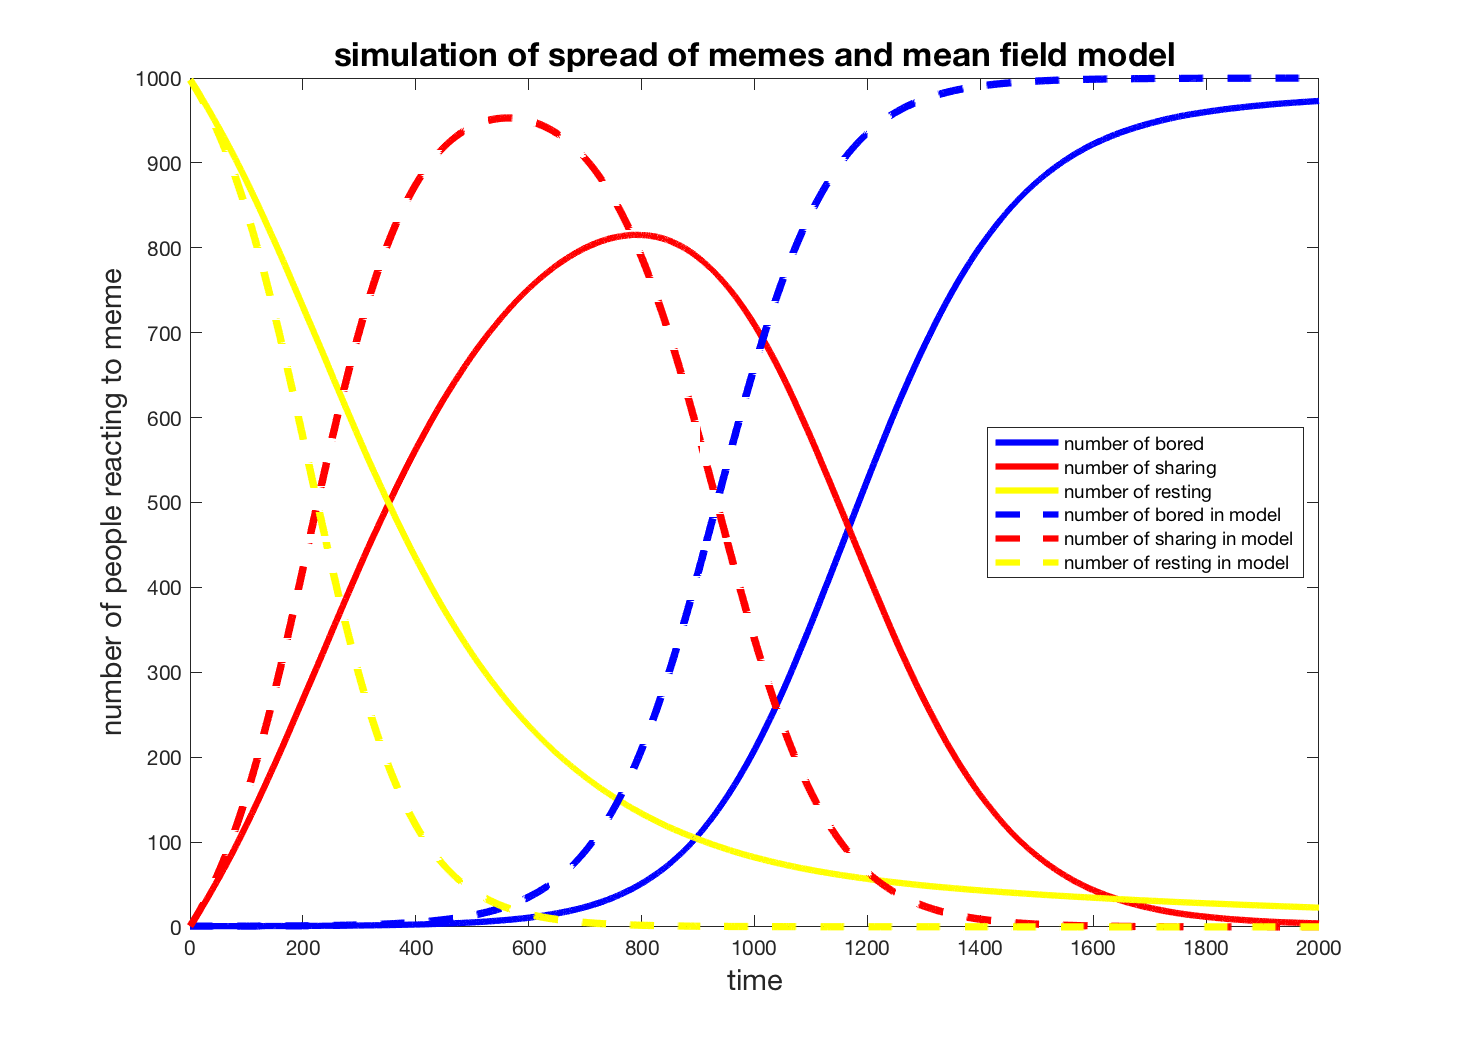
\includegraphics[width = 16 cm, height = 13cm]{memes_withmodel1000.png}
\caption{simulation of spread of memes showing number of bored, sharing, resting person over time with mean field model}
\label{fig:meme_sim_model}
\end{figure}

\begin{figure}[H] %phase transition
\centering
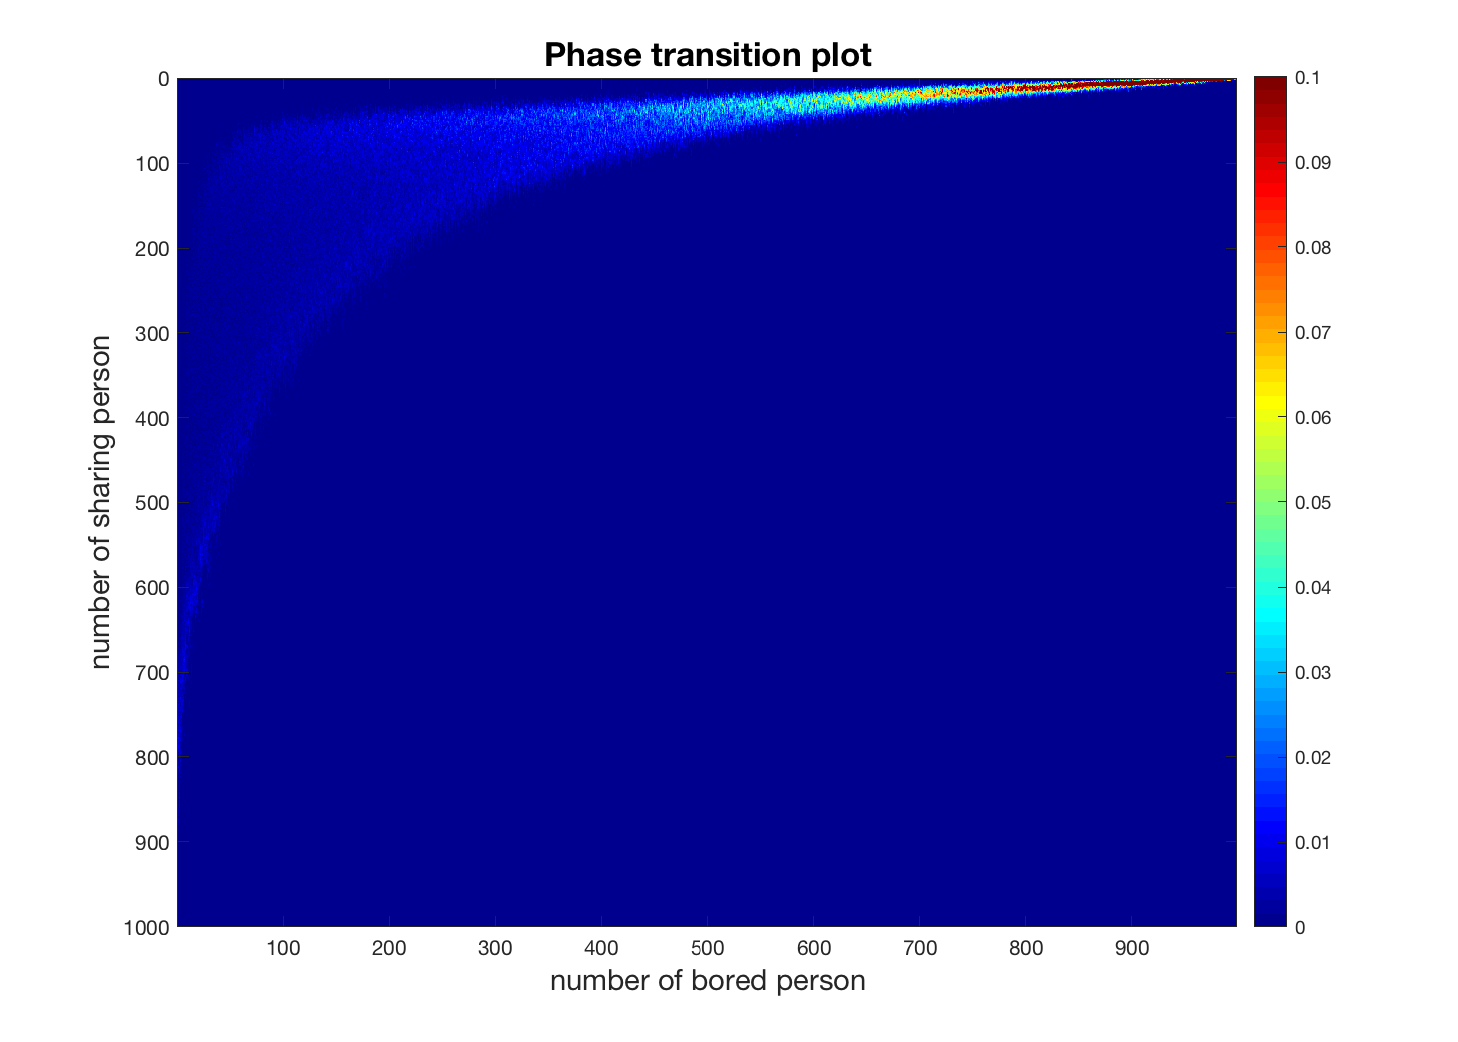
\includegraphics[width = 16 cm, height = 13cm]{phasetransition.png}
\caption{phase transition of total sharing person with simulation with t = 1000 and different B(0) condition}
\label{fig:meme_phase_transition_1}
\end{figure}

\begin{figure}[H] %result plot of individual
\centering
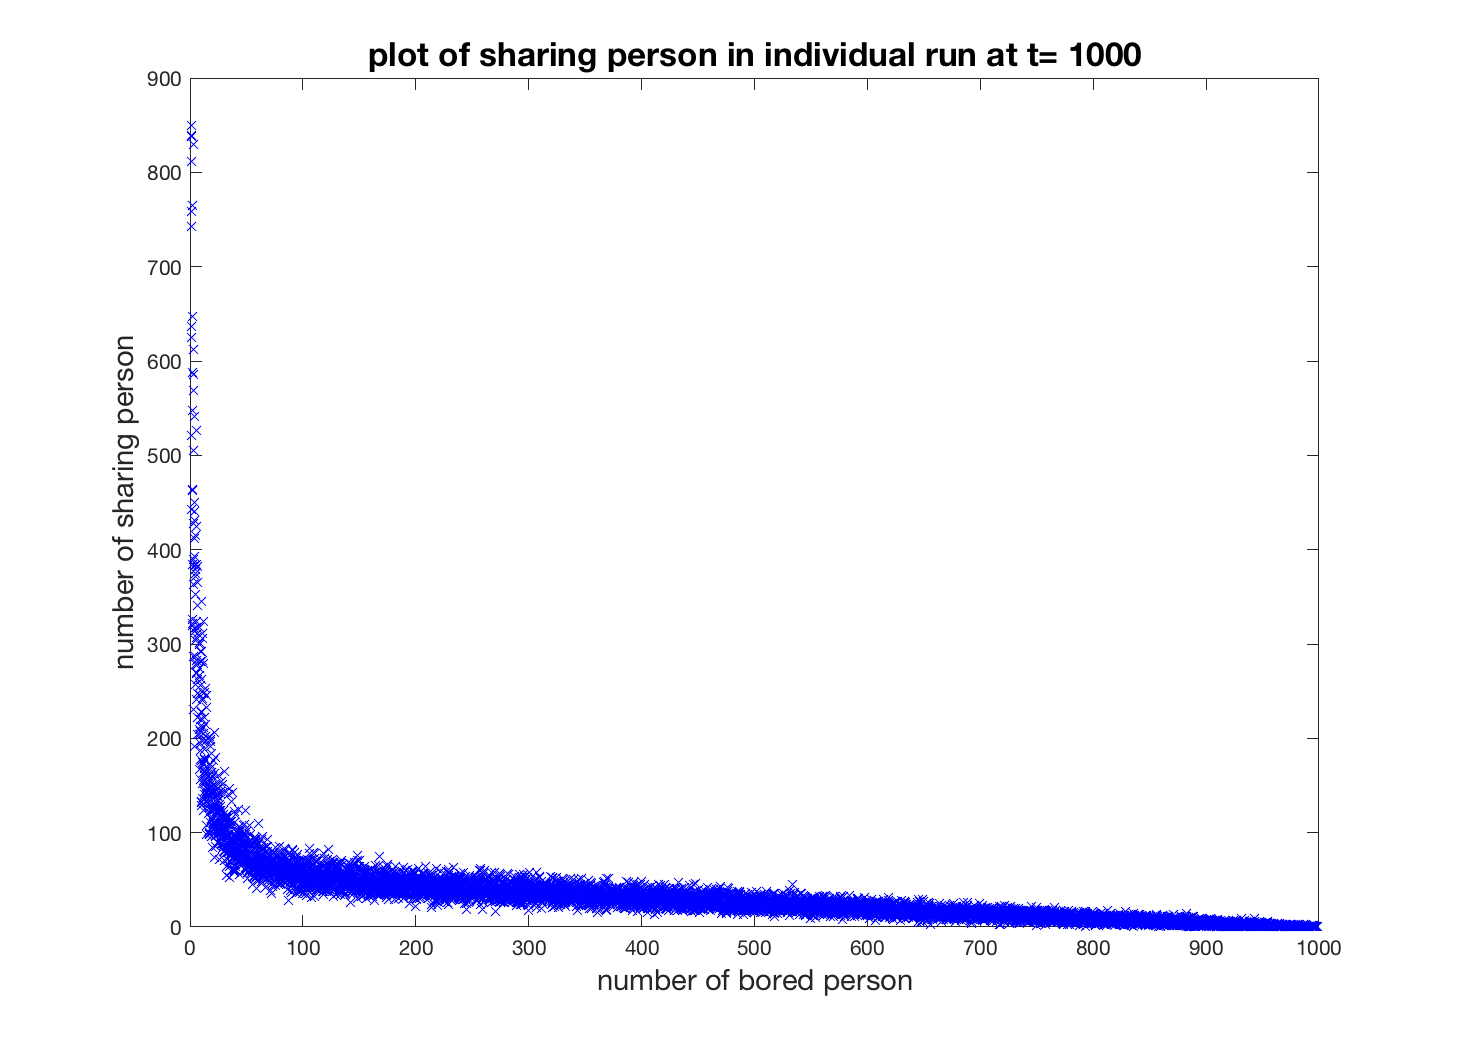
\includegraphics[width = 16 cm, height = 13cm]{indi_phase.png}
\caption{plot of sharing person in individual runs at t =1000 for 100 simulations of B0 = 1:1:999}
\label{fig:meme_phase_transition_indi}
\end{figure}

To find the probability of at least 25\% of the populations share a meme. I run the model with B(0) = 1:1:999 for 100 times to final time = 1000. and plot the probability in a heat map. 

\begin{figure}[H] %result plot of individual
\centering
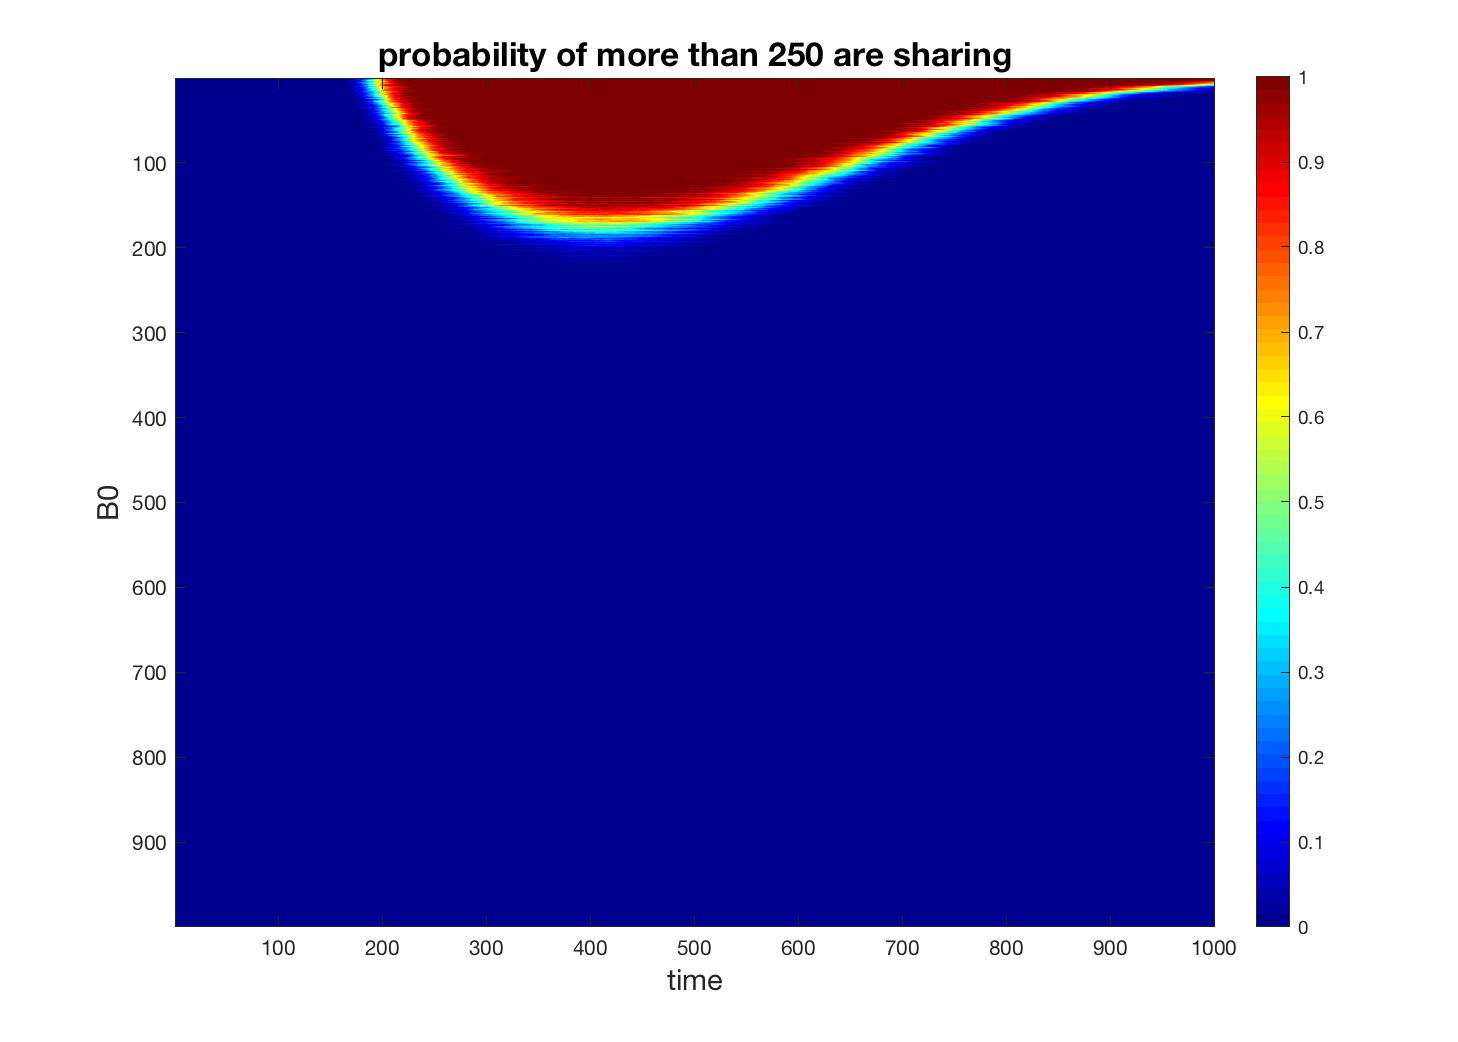
\includegraphics[width = 16 cm, height = 13cm]{probability250_100sim.png}
\caption{probability of more than 250 people are sharing with different B0 and time from 0 to 1000}
\label{fig:probability250}
\end{figure}

\newpage


%%%%%%%2.2 with different rules on bored 

\subsection{changed the condition of a bored person}
One condition was added to the bored person. A bored person will pick on person a random from the population with probability of q. If that person is resting then the bored person will become resting. otherwise she will continue to be bored. It was simulated in matlab for 1000 times with a population of 1000 to time = 2000 and at the same time plot together with the mean field model. The results were very different compared to the previous simulation. It seems that the model shows oscillation of bored person and sharing person over time but not in the simulation. In the model, we allow decimals for the number of persons. that's why the number of bored persons can slowly increase. In the simulation, it started with 1 bored person, and if that person meets someone at rest with probability of q. Then this bored person will be resting too. With this condition, a bored person soon finds a person at rest and then bored persons will be 0. The sharing person will increase gradually as a resting person will find a meme with p = 0.001. In the simulation one person can only be in one of the three states, that's why the simulations shows different results. 

\begin{figure}[H] %rmeme2 1000 runs
\centering
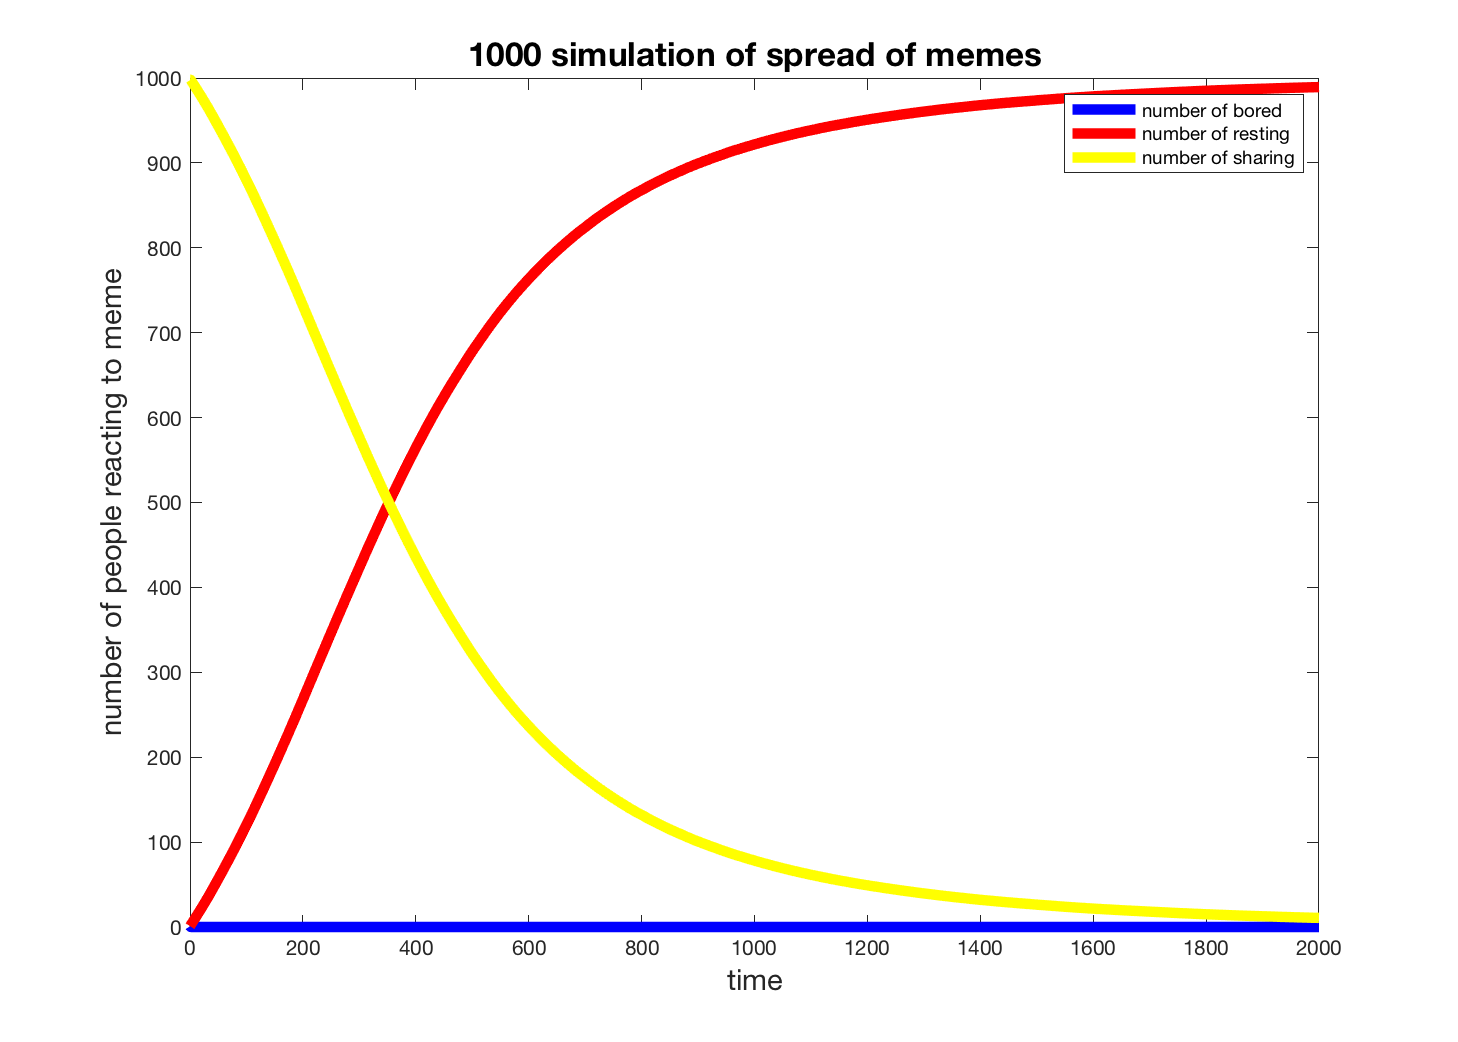
\includegraphics[width = 16 cm, height = 13cm]{memes2_sim_1000times.png}
\caption{100 simulations of memes with different rules for bored person over t = 2000  }
\label{fig:meme2sim1000}
\end{figure}

\begin{figure}[H] %meme2 1000 runs with model
\centering
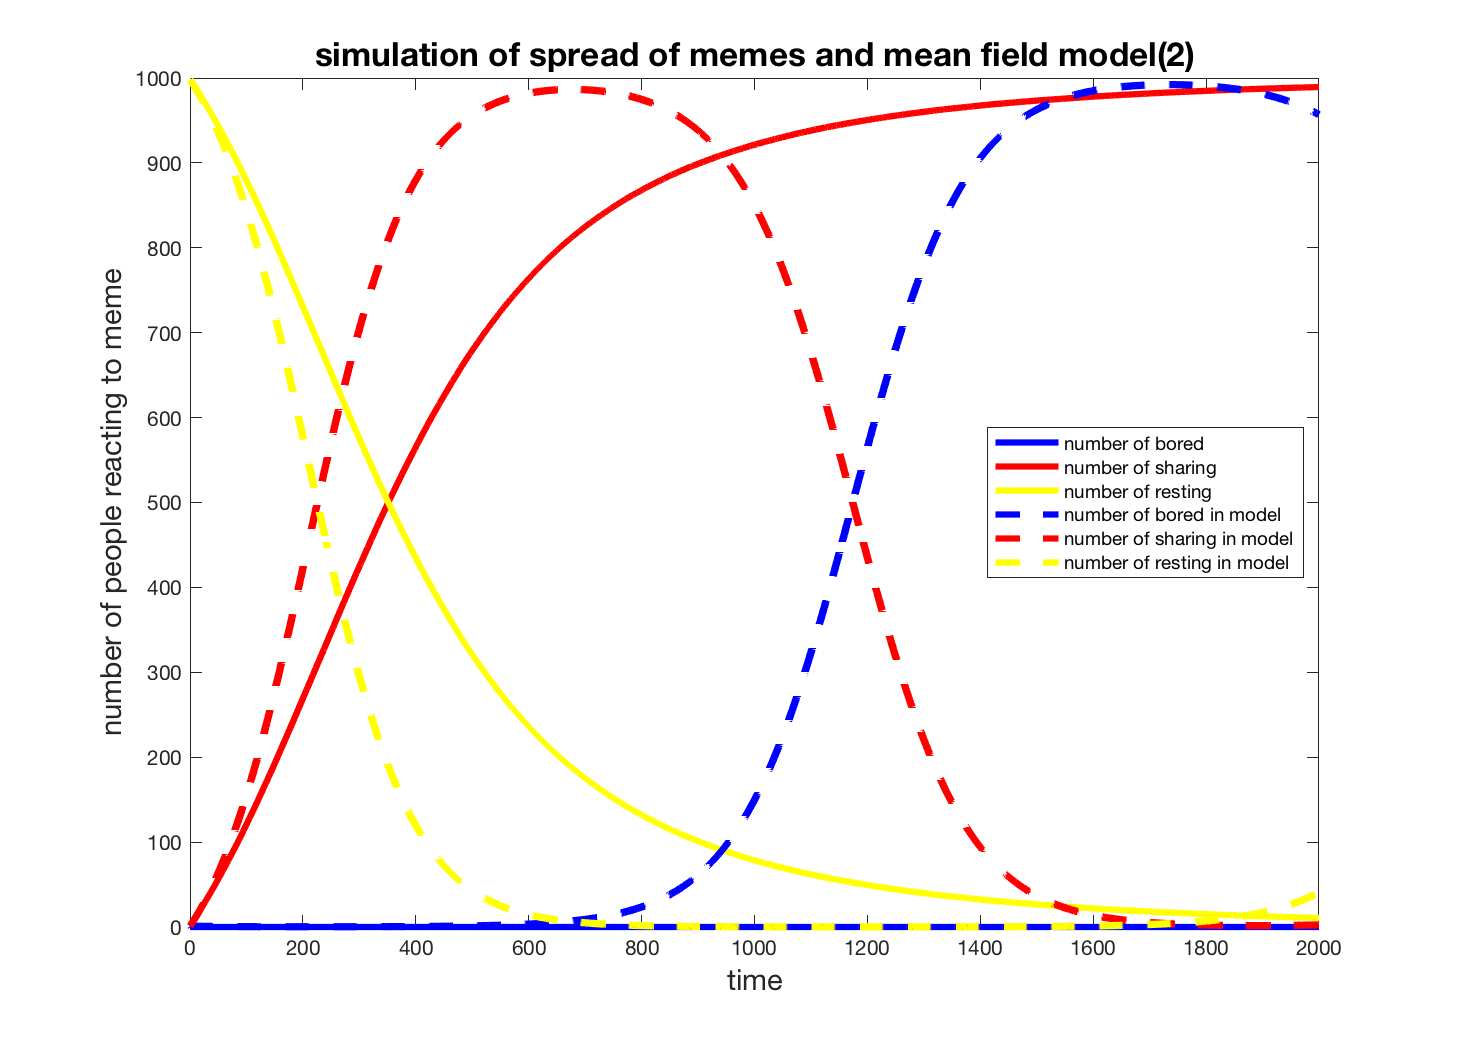
\includegraphics[width = 16 cm, height = 13cm]{memes2_withmodel1000.png}
\caption{100 simulations of memes with different rules for bored person over t = 2000  with mean field model plot}
\label{fig:meme2sim1000model}
\end{figure}

A phase transtion over q = 0.01:0.01:1 was made for the simulation. it is interesting to see that with probability q a person interact with another either to share or transtion from bored to rest. from q = 0.01 to q = 0.1, the total number of sharing persons at t = 1000 increase rapidly and almost everyone was sharing in the end when p $>$ 0.1. 
\begin{figure}[H] %meme2 phase
\centering
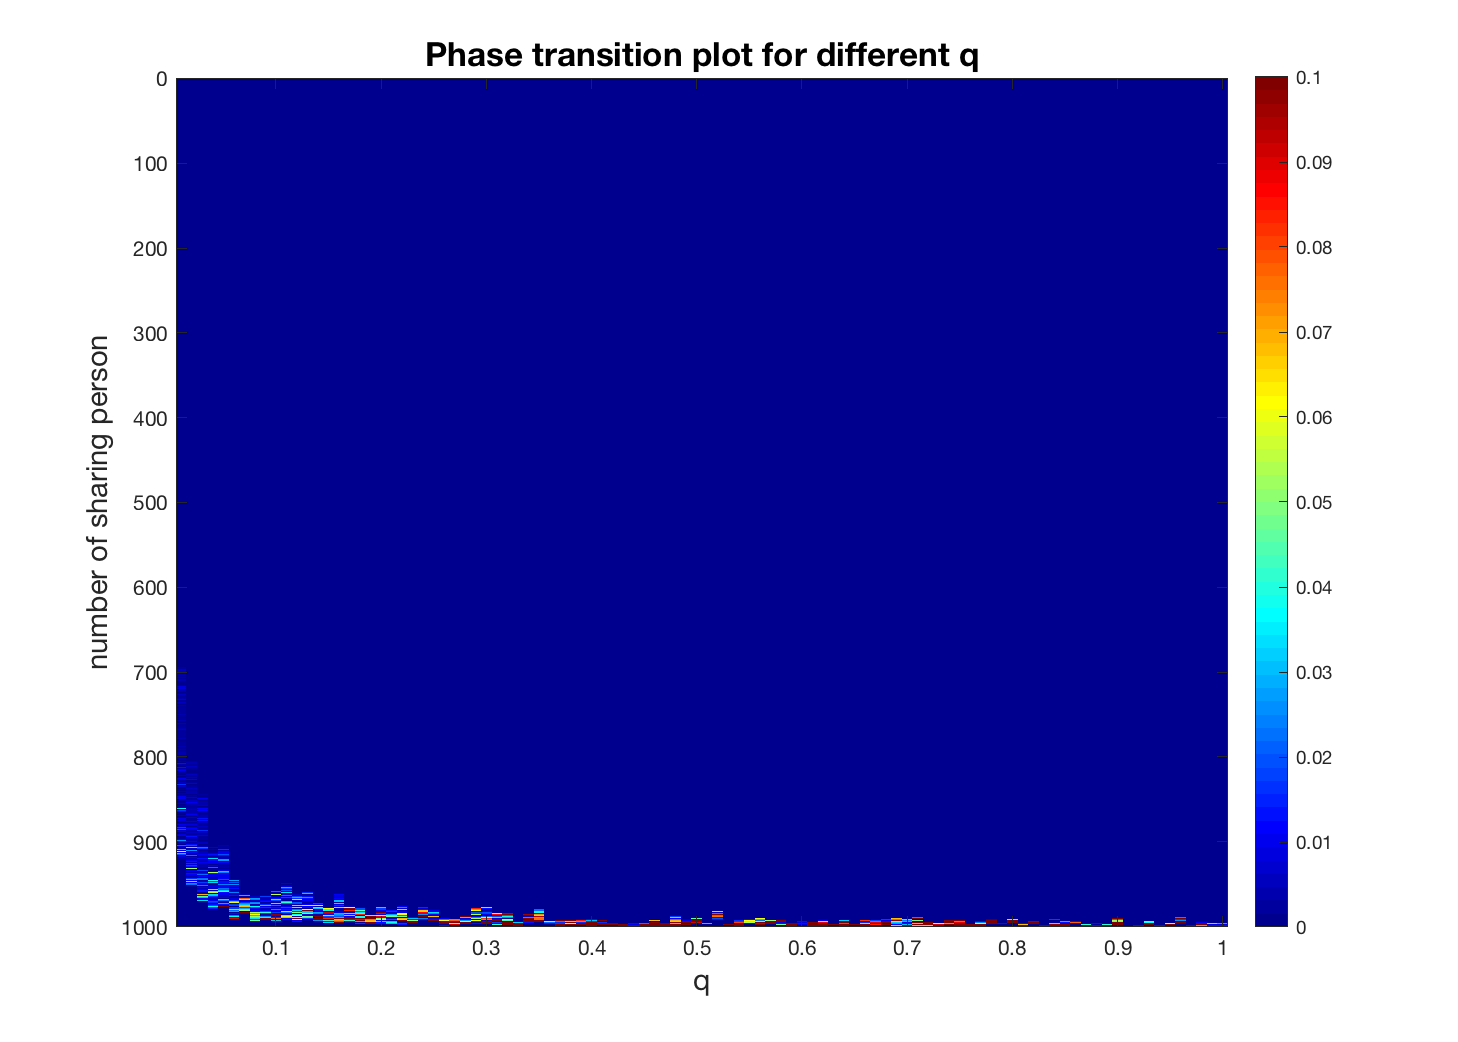
\includegraphics[width = 16 cm, height = 13cm]{phasetransition2.png}
\caption{phase transition of total sharing person with simulation with t = 1000 and different q condition }
\label{fig:phasetransition2}
\end{figure}

\begin{figure}[H] %meme2 phase indi
\centering
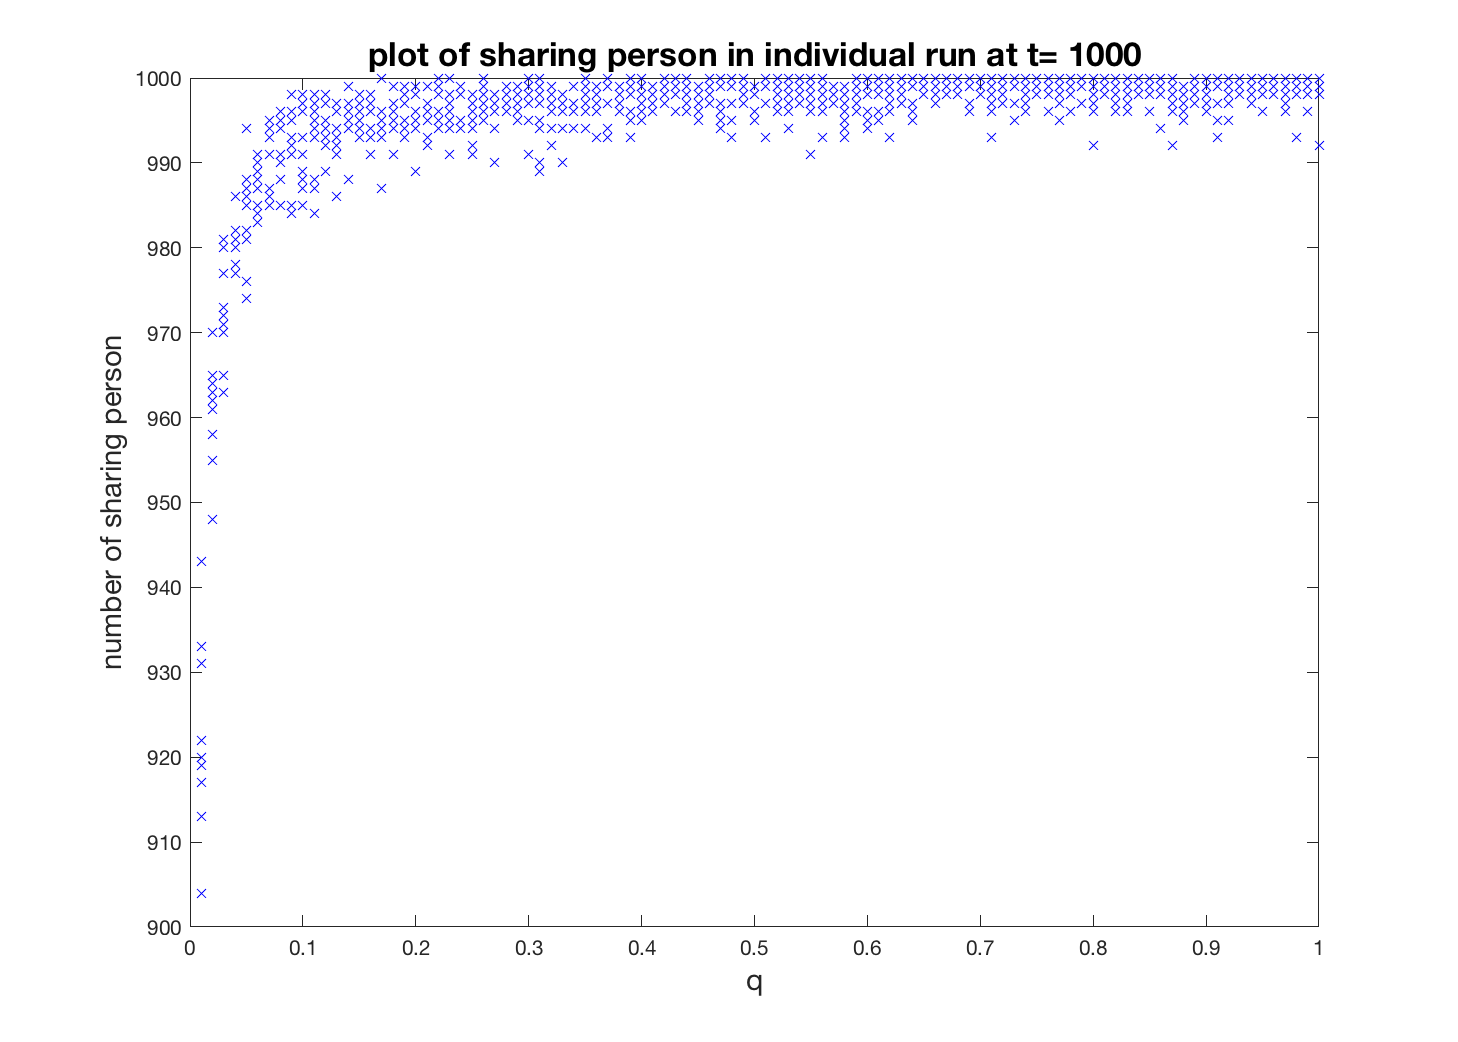
\includegraphics[width = 16 cm, height = 13cm]{indi_phase2t1000withq.png}
\caption{plot of sharing person in individual run at t = 1000 }
\label{fig:phasetransition2indi1000}
\end{figure}

\subsection{simulate on grids of 40x40 for spread of memes}
In this part, we use the model above and in 2.2 to simulate that the person can only interact with the neighbours. the boundary conditions are set to be periodic. so that it goes from left to right, right to left, up to bottom, and bottom to up. After several runs. it can be observed that the number of sharer are increasing steadily. while the number of bored people tend to remain around at 1.the only way that bored person increase is that a sharing person meets a bored person. in theory the probability is p = 1* 0.01*(1/1600). For the majority resting population, with a chance of 0.001 to discover a memes and become a sharer. in the initial state, there were 1588 resting people, that means that in theory 1.5 people will become a sharer. That's why it grows very fast, when t gets to 1000. almost everyone is sharing. 

\begin{figure}[H] %meme2 phase indi
\centering
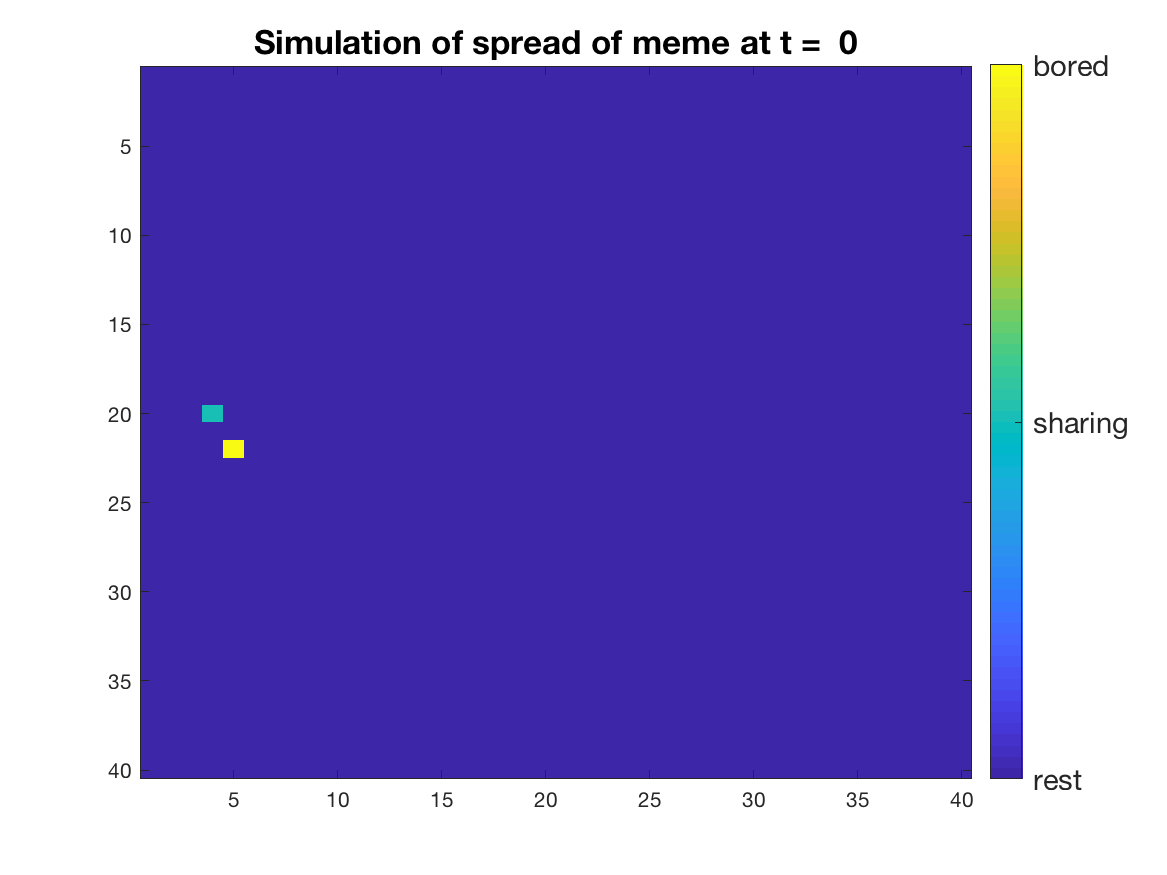
\includegraphics[width = 16 cm, height = 13cm]{memegrid.png}
\caption{initial condition for simulation}
\label{fig:memegrid0}
\end{figure}

\begin{figure}[H] %meme2 phase indi
\centering
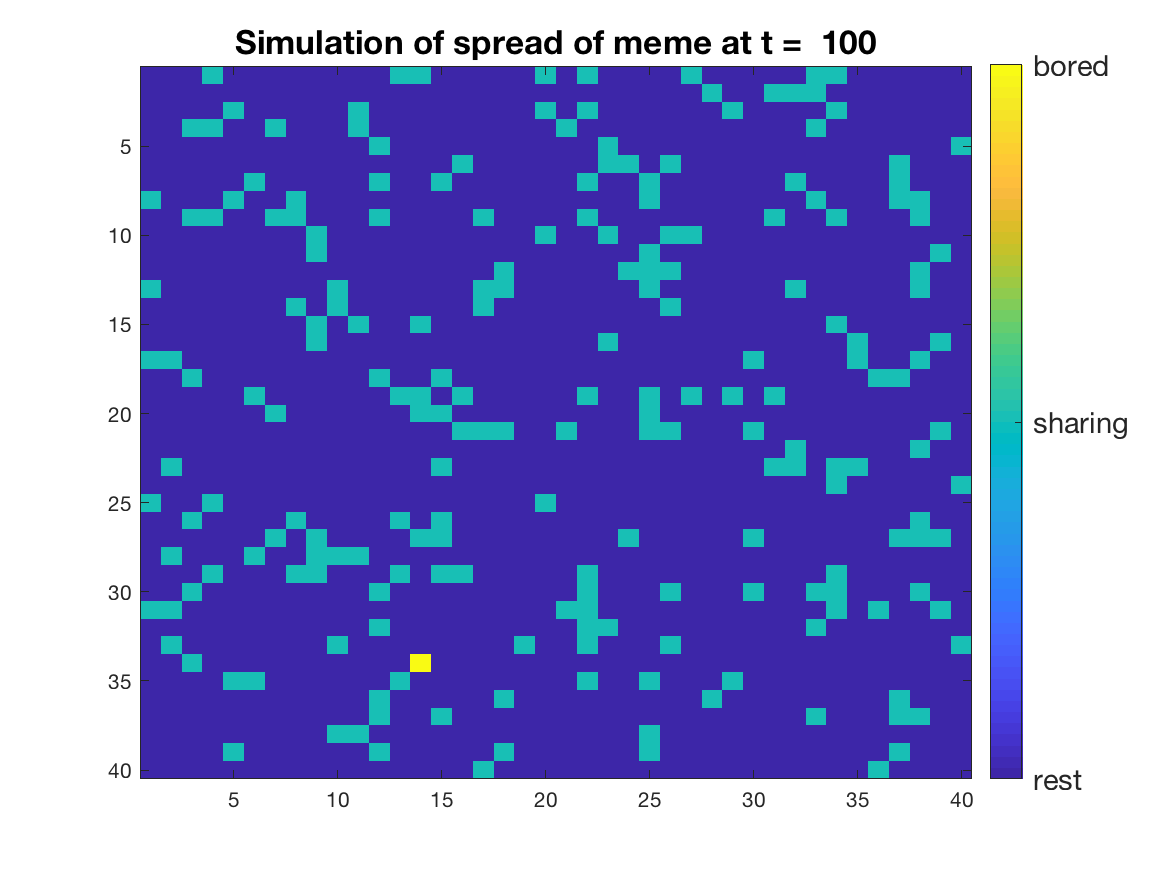
\includegraphics[width = 16 cm, height = 13cm]{memegrid100.png}
\caption{simulation of spread of meme to t = 100}
\label{fig:memegrid100}
\end{figure}

The video of the simulation can be found at 
\url{<https://www.youtube.com/watch?v=WMfI2P52ros>}

%%%%%%%%%%%%%%%%%%
%%%%%%%%%%%%%%%%%
%%%%%%%%%%%%%%%%%appendix
\newpage
\section{Appendix}

\subsection{1firing brain code in matlab}
\singlespacing
\begin{itemize}
\item {\large simulate single time of fire brain}
\lstinputlisting{firebrain1.m}
\vspace{1cm}

\item {\large transition function}
\lstinputlisting{transit.m}
\vspace{1cm}

\item {\large initial state}
\lstinputlisting{random_start.m}
\vspace{1cm}

\item {\large simulate 100 times of firing brain}
\lstinputlisting{firebrain1_simulate100.m}
\vspace{1cm}

\item {\large cell that move forward at one cell per time preserving the same shape}
\lstinputlisting{task2_1.m}
\vspace{1cm}

\item {\large cell that move forwad at one cell per time, launching other shapes behind them}
\lstinputlisting{task2_2a.m}
\vspace{1cm}

\item {\large move forward at a rate of less than one cell per time step}
\lstinputlisting{task2_3.m}
\vspace{1cm}

\item {\large oscillate shape}
\lstinputlisting{task2_4.m}
\vspace{1cm}


\item {\large my cellular automata}
\lstinputlisting{reproduceown.m}
\vspace{1cm}

\item {\large my cellular automata transit}
\lstinputlisting{transitown.m}
\vspace{1cm}


\end{itemize}



\subsection{Spread of memes}

\singlespacing
\begin{itemize}

\item{\large simulation of spread of memes}
\lstinputlisting{sim_meme1.m}
\vspace{1cm}

\item{\large run single spread of memes }
\lstinputlisting{runmeme.m}
\vspace{1cm}

\item{\large mean field model}
\lstinputlisting{sim_meme_model.m}
\vspace{1cm}

\item{\large phase transition}
\lstinputlisting{sim_meme_phase.m}
\vspace{1cm}


\item{\large probability for at least 25\% are sharing}
\lstinputlisting{plargethan250.m}
\vspace{1cm}


\item{\large simulation of spread of memes with new rules}
\lstinputlisting{sim_meme2.m}
\vspace{1cm}

\item{\large run single spread of memes }
\lstinputlisting{runmeme_newbored.m}
\vspace{1cm}

\item{\large mean field model}
\lstinputlisting{sim_meme_model2.m}
\vspace{1cm}

\item{\large phase transition for new rules}
\lstinputlisting{sim_meme_phase2.m}
\vspace{1cm}

\item{\large lattice simulation for memes}
\lstinputlisting{memegrid.m}
\vspace{1cm}

\item{\large transition function for memes}
\lstinputlisting{transit_meme.m}
\vspace{1cm}


\end{itemize}


\end{document}